\chapter{Longest-Chain Consensus}
\section{A Tale of Two Protocol Paradigms}
Chapter 7 was about the Tendermint protocol (for state machine replication), and its optimal
fault-tolerance in the partially synchronous model (with consistency always and liveness
eventually). This was the culmination of our six-chapter boot camp on classical consensus
protocols. Most of what we talked about was figured out by brilliant computer scientists
in the 1980s. (Tendermint is a 21st-century protocol, but heavily influenced by the classic protocols from the 1980s and 1990s.1
) As you may know, the most famous blockchain
protocol of them all (Bitcoin) is based on a consensus protocol that does not at all resemble
those that we've been discussing thus far. In the blockchain world, there are currently two
prevalent paradigms for consensus protocols, “BFT-type” and “longest-chain” protocols.

\subsection{Category 1: BFT-type Protocols (e.g., Tendermint)}
Protocols like Tendermint are often called BFT or BFT-type protocols; the “BFT” stands
for “Byzantine fault tolerant.” The first shared property of these protocols is that they all
look similar from 30,000 feet, with multiple stages of voting and some analog of quorum
certificates. This ensures that a node commits to a new block only after it can be certain
that (assuming not too many Byzantine nodes) no other honest node will ever commit to
any other version of that block.\\
By design, under appropriate assumptions (such as $f < \frac{n}{3}$, where $f$ and $n$ denote
the number of Byzantine and total nodes, respectively), BFT protocols do not suffer from
“forks”—there will never be two different blocks committed by honest nodes at the same
block height. If there ever is a fork in a BFT-type protocol (either due to a buggy implementation or more Byzantine nodes than expected), it’s not at all clear how to resolve the
fork from within the protocol.\\
Because BFT-type protocols favor consistency over liveness (when the network is poor
or under attack), when they fail (for whatever reason), they typically fail by stalling (i.e.,
not confirming any new blocks of transactions for a prolonged period of time). You do not
typically hear, for instance, about double-spend attacks caused by the rollback of thought-to-be-finalized blocks.
\subsection{Category 2: Longest-Chain Protocols (e.g., Bitcoin)}
If you've watched even a 20-minute video on Bitcoin at some point in your life, you already
know there’s a second category of blockchain consensus protocols, namely longest-chain
protocols. The longest-chain consensus was invented by Nakamoto and first described in the
Bitcoin white paper.
Conceptually, longest-chain protocols are radically different from BFT-type protocols:
\begin{enumerate}
    \item There is no explicit voting - each block (along with an explicit pointer to a predecessor block) is proposed unilaterally by some node.
    \item Because there's no waiting for quorum certificates, forks - two (potentially conflicting) blocks that claim a common predecessor - can easily arise in the normal course of business (either due to Byzantine nodes or network delays). With potentially frequent forks, such a protocol can function only if it has an in-protocol way of automatically resolving the ambiguity introduced by a fork. This is done by - wait for it - always resolving forks in favor of the longest chain of blocks. (We'll get into all the protocol details and nuances starting in the next section.)
    \item Under embracing forks and resolving them in the protocol, longest-chain protocols favor liveness over consistency when there's a communication breakdown between nodes. Accordingly, in practice, longest-chain protocols tend to fail by violating consistency (with nodes disagreeing on which blocks have been finalized, leading to thought-tobe-confirmed blocks getting rolled back) rather than by stalling. ${ }^{5}$ Such consistency violations can enable "double-spend" attacks. For example, suppose a blockchain transaction carries the payment for an expensive physical good like a Tesla. Once the Tesla dealer regards the transaction as confirmed, they let the buyer drive off in their new car. If that transaction later gets rolled back, the buyer effectively gets a full refund even though they still have the car.
\end{enumerate}


\section{Longest-Chain Consensus}
\subsection{Preamble}

The version of the longest-chain consensus described in this chapter may differ from what you had in mind.\\

\noindent
\textbf{This chapter: permissioned setting, PKI assumption.} Throughout this chapter, we will continue working in the permissioned setting with the PKI assumption (with an a priori known set of nodes running the protocol, each with a private key and a known-to-all corresponding public key). One reason for this is the continuity of all of the chapters thus far. Another reason is that many of the novel ideas in and properties of longest-chain consensus manifest already in this setting.

That said, the longest-chain consensus's biggest claim to fame is its shockingly graceful extension to the "permissionless" setting in which the protocol has no idea what nodes are running it. The next chapter (Chapter 9) is all about permissionless longest-chain consensus (specifically, the "proof-of-work" version used in Bitcoin).\\

\noindent
\textbf{Looking ahead toward the Bitcoin protocol.} As I've said many times, this chapter series is focused on principles of blockchain design and analysis rather than on specific blockchain protocols per se. And if you study Bitcoin for Bitcoin's sake, for example, you generally wind up conflating multiple independent innovations. We'll take care to unbundle these innovations in this chapter series, both because of the mental clarity that it affords and because the separate pieces can be remixed with other ideas to design other interesting blockchain protocols.\\
A consensus protocol lays down the law about which of the proposed blocks are the ones that count (and about their ordering). A conceptually distinct question is about which nodes can participate (e.g., by proposing a new block or voting on a previously proposed block). It's easy to come up with answers to this question in the permissioned setting (with the PKI assumption) - for example, by letting all nodes vote and having nodes take round-$r$obin turns acting as the block proposer. It's much harder in the permissionless setting because the protocol has no idea which nodes are running it. The second big innovation in Bitcoin (in addition to longest-chain consensus) is an effective way of selecting block proposers in longest-chain consensus in the permissionless setting, using an idea known as "proof-of-work."\\
In this chapter series, we'll keep these two questions (which blocks count? Who participates in block production?) as separate as possible. They will interact a little bit at their edges, though, as we'll see (see page 13).\\

\noindent
\textbf{Permissioned + PKI vs. proof-of-work vs. proof-of-stake implementations.} Some readers may enter this chapter with the mindset of permissioned consensus (e.g., those coming in directly from chapters 2-7) while others may be strongly influenced by famous permissionless blockchain protocols that they've read about (e.g., Bitcoin and Ethereum). I'm going to try to have my cake and eat it too, by addressing both audiences at the same time.

The plan is for the main narrative of this chapter to focus squarely on longest-chain consensus in the permissioned setting (with the PKI assumption) but with frequent side comments and forward pointers about how to interpret that narrative in the content of permissionless blockchain protocols. We'll provide interpretations both for the proof-of-work implementation described in chapter 9, and the "proof-of-stake" implementation covered in chapter 12. Don't worry about it if you've never heard about approaches to "sybil-resistance" like proof-of-work or proof-of-stake - the main narrative of this chapter assumes nothing other than familiarity with permissioned protocols for state machine replication (as covered in the preceding chapters).\\

\noindent
\textbf{Remember the Dolev-Strong protocol?} Another reason to keep looking forward toward permissionless implementations is that in the setting of this chapter (permissioned setting with the PKI assumption), the longest-chain consensus is strictly dominated by an SMR protocol that we analyzed way back in Chapter 2 - the (iterated) Dolev-Strong protocol. That

${ }^{6}$ The combination of longest-chain consensus with proof-of-work block proposer selection, as introduced in Bitcoin, is sometimes called "Nakamoto consensus." protocol has some impressive provable guarantees - consistency and liveness even when $99 \%$ of the nodes are Byzantine-provided you're willing to make a bunch of assumptions: the permissioned setting, the PKI assumption, and the synchronous model (with an a priori known bound $\Delta$ on the maximum message delay).

As we'll see (Section 8.11), longest-chain consensus loses consistency in the partially synchronous setting and for this reason is studied primarily in the synchronous setting. Here, the protocol can guarantee consistency and liveness provided at most $49 \%$ of the nodes are Byzantine (see Theorems ?? and 10.1). It's not trivial to design a protocol with such guarantees (nor is it easy to prove that longest-chain consensus does, in fact, offer them), but one has to concede that - in the permissioned setting, with the PKI assumption, in the synchronous model - there's really no reason to use longest-chain consensus instead of simply running the Dolev-Strong protocol once for each block (with rotating or randomly chosen block proposers/senders).

Thus, it's only once we pass to the permissionless setting that the longest-chain consensus allows us to reach goals that we don't otherwise know how to achieve. This chapter is, therefore, best viewed as a stepping stone toward the proof-of-work and proof-of-stake implementations of longest-chain consensus studied in chapters 9 and 12, rather than as an end unto itself. But I promise that I'm not wasting your time - the key points in this chapter are all essential even for the reader who cares only about understanding permissionless longest-chain consensus.

\subsection{Protocol Description}

Our description of longest-chain consensus has three scenarios simultaneously in mind:\\

(PKI) Permissioned setting, PKI assumption.

(PoW) Permissionless setting, proof-of-work sybil-resistance.

(PoS) Permissionless setting, proof-of-stake sybil-resistance.

If you're unfamiliar with any permissionless blockchain protocols, ignore all comments about scenarios (PoW) and (PoS) - all will become clear in chapters 9 and 12, respectively.

\noindent
\textbf{An underspecified version.} Let's start with an abstract and underspecified description of the longest-chain consensus, before interpreting it in each of the three scenarios above.

\nt{
\begin{center}
    \textbf{Longest-Chain Consensus (Abstract Version)}
\end{center}
\noindent
(1) Start with a hard-coded genesis block $B_{\text {gen }}$.\\
\noindent
(2) In each "round" $r=1,2,3, \ldots$ :\\

\hspace{0.4cm}(2a) Choose one node $\ell$ as the leader of round $r$.

\hspace{0.4cm}(2b) Node $\ell$ proposes a set of blocks, each specifying a single predecessor block.}

\begin{figure}[h]
    \centering
    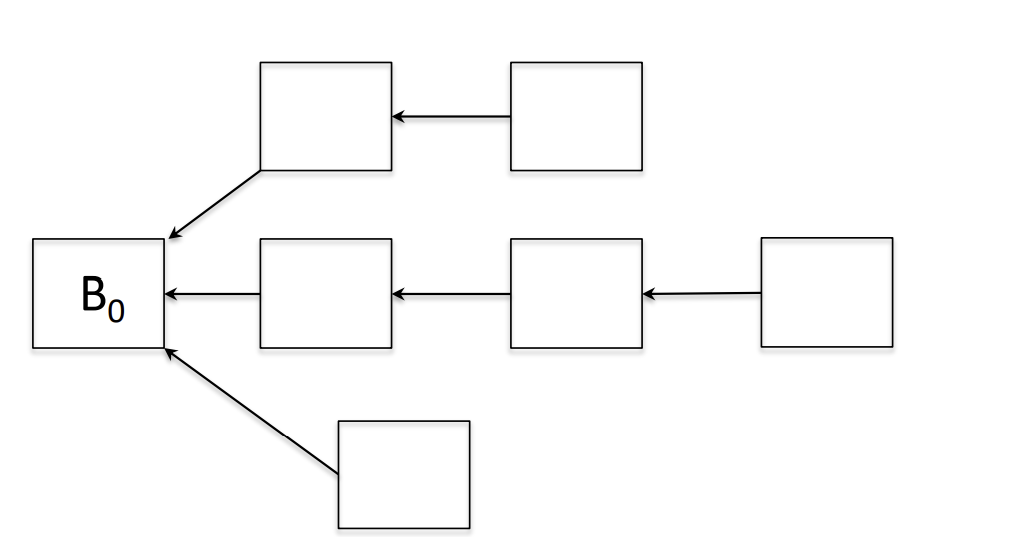
\includegraphics[scale = 0.5]{figures/f22.png}
    \caption{The blocks produced in longest-chain consensus can be visualized as a tree, directed toward the genesis block (root).}
    \label{fig:mesh1}
\end{figure}\\
We'll supply more details below, but already at this level of specification we can fruitfully visualize the data structure produced by the nodes running the protocol as an in-tree - a tree (in the sense of an acyclic connected graph) in which all edges are directed back toward the root (Figure 8.1). For us, the genesis block acts as the tree's root, and each directed edge corresponds to one block's naming of its predecessor. ${ }^{7}$ When the protocol is first fired up, this in-tree consists solely of the genesis block; as the rounds go by, nodes running the protocol continue to grow this in-tree (with each leader adding a new batch of vertices, each with out-degree 1). Note that, as promised, forks (a block named as the predecessor of multiple blocks, or equivalently a vertex with in-degree greater than 1) are embraced as part of normal operation.\\

\noindent
\textbf{The genesis block.} Every longest-chain protocol has baked into it a genesis block that gets the party started. There are no transactions in the genesis block, but it is an eligible predecessor for any block that might be created later. Just as each node is born knowing the protocol code (and, in the PKI setting, its private key and all nodes' public keys), each node should be thought of as born knowing the genesis block.\\

\noindent
\textbf{What's a "round"?} Each iteration of longest-chain consensus, each with a single leader node who's granted the power to add to the current blockchain is called a round. The meaning of a round depends on which scenario we're talking about. In scenarios (PKI) and (PoS), we'll assume a shared global clock (as in the synchronous model) and each round will correspond to a time interval of a fixed length. For example, round 1 might be the first 10 seconds, round 2 the next 10 sections, and so on. We've seen this idea before (in scenario (PKI)), for instance, in the iterated Dolev-Strong protocol in chapter 2 and the Tendermint protocol in chapter 7.\\
Interestingly, in scenario (PoW), rounds will not correspond to fixed periods of time (except in a loose average sense), and more generally, there's only minimal reliance on a shared notion of time. Rather, rounds are defined in a purely event-driven way. Readers who know how proof-of-work works - with block producers racing to be the first to solve a difficult cryptographic puzzle - may already see what I mean by "event-driven." Every time some block producer gets lucky and solves a puzzle (the event of interest), we'll call that the next round.\\

\noindent
\textbf{How is the leader chosen?} Each round has a single node that acts as the leader. The abstract description above is silent on how this happens in step (2a), and the answer depends on which scenario we're looking at.\\
The simplest scenario is (PKI). We could reuse our approach from chapters 2 and 7 of round-$r$obin rotating leaders. E.g., if there are 100 nodes and it's currently round 117, node 17 is the leader. Alternatively, and better for longest-chain consensus (as we'll see), leaders could be chosen (pseudo)randomly - for example, using a hash $h(117)$ of the current time step rather than the time step 117 itself to identify the current leader. Either way, assuming that each round has a fixed length and that all nodes share a global clock, they all automatically know what round it is, and in the permissioned setting they all then know which node is the leader at any given time.\\
You can, at a high level, think of scenario (PoS) as similar to the second approach in scenario (PKI), with leaders chosen randomly. A twist is that leaders will be not be selected uniformly at random, but rather with probability proportional to the amount of stake (in the blockchain's native currency) that a node has locked up in a designated smart contract. E.g., if $10 \%$ of the total stake locked up in the contract is owned by node $i$, then in any given round, node $i$ has a 1 in 10 chance of being chosen as the round's leader. (We'll talk about all the nuances of implementing this idea in chapter 12.)
Scenario (PoW) is similar to (PoS) except that a node is effectively selected as a leadermeaning it's the first node to solve a hard cryptographic puzzle - with probability proportional to the amount of computational power that it contributes to the protocol (rather than to the amount of locked-up stake).\\

\noindent
\textbf{What can the leader do?} Once a node is selected as the leader of a round (in step (2a)), in step (2b) that node gets to create some number of blocks. Here a block is, as usual, an ordered sequence of transactions (which were presumably submitted to nodes earlier by the clients participating in the SMR protocol). However many blocks that leader creates, it must specify a unique predecessor block for each of those blocks. (Any block that specifies zero or more than two valid predecessors is automatically considered invalid by all honest nodes. Looking ahead, an honest leader will be instructed to create exactly one block; it's Byzantine nodes that might create several.) The leader is always in a position to do this - if nothing else, it can use the (commonly known) genesis block as a predecessor.

As we'll see below, exactly what the leader is capable of doing will depend on which of the scenarios we're in (e.g., the leader is most highly constrained in scenario (PoW)) - this is the part of longest-chain consensus in which there is inevitably interaction between the details of the consensus protocol and the method by which nodes are selected to participate.

The use of explicit predecessors is a departure from BFT-type protocols like Tendermint in which, assuming less than a third of the nodes are Byzantine, there will be only one block at each block height (because quorum certificates are required for block finalization, and by the quorum intersection property). Because there's only going to be one block \#8, one block $\# 9$, one block \#10, and so on, there's no need to explicitly name a predecessor-everyone knows that the predecessor is the (unique) block at the previous height. In longest-chain consensus, any leader can create a fork if it wants (e.g., by proposing multiple blocks, all with the same predecessor). Thus there may be multiple blocks at each block height, effectively competing for eventual finalization. This renders explicit predecessors necessary - if there are multiple blocks at height 8, a block at height 9 needs to specify which one it views as the preceding block.

\section{Five Assumptions}

The goal of this chapter is to show that longest-chain consensus satisfies consistency and liveness in the synchronous model provided at most $49 \%$ of the nodes are Byzantine. We'll carry out this analysis under five assumptions, detailed and discussed next.

\subsection{Assumptions About the Genesis Block}

The first assumption is a trusted setup assumption - meaning an assumption that we take on faith, kicking the can down the road as to how it might be enforced. Specifically, we assume that no nodes are privy in advance to the description of the protocol's genesis block-nodes only learn the name of that block at the moment the protocol commences. (E.g., the genesis block can't have been chosen by some Byzantine node in advance.)
\nt{
\begin{center}
    \textbf{Assumption (A1)}
\end{center}
\noindent
(A1) No node has knowledge of the genesis block prior to the deployment of the protocol.
}

As a trusted setup assumption, we'll make no effort to enforce it within the protocol itself (regardless of which of the three scenarios we're in). When deploying a longest-chain protocol, a good faith gesture is to include a genesis block that references verifiable information that could not have realistically been predicted well in advance of the protocol's deployment. This assumption will show up in an important (but subtle) way in our proof of Theorem 8.7.1.

\subsection{Assumptions About Leader Selection}

We'll also need two assumptions about how leader selection works in step (2a) of longestchain consensus. These are not trusted setup assumptions, and we'll need to make sure that a concrete implementation of longest-chain consensus enforces them. ${ }^{9}$

\nt{
\begin{center}
    \textbf{Assumption (A2)}
\end{center}
\noindent
(A2) It is easy for all nodes to verify whether a given node is the leader of a given round.}

The second assumption asserts that each round's leader selection should be verifiable. This means two things: the round's selected leader can easily prove it is in fact the leader; and no other node can trick honest nodes into thinking it's actually the leader.

Happily, assumption (A2) takes care of itself in all the scenarios that we're interested in. In scenario (PKI), imagine that leaders rotate in round-robin order, e.g. with node 17 automatically the leader of round 117 (assuming $n=100$ ). Imagine further that every message sent by an (honest) node is signed by the sender and annotated with the round it belongs to. Because of the PKI assumption, node 17 and only node 17 will be in a position to send messages as the leader in round 117 (if a round-117 message that is supposed to be from the round's leader is not signed appropriately, all honest nodes ignore the message). The same reasoning holds for pseudorandomly chosen leaders.

In scenario (PoS), leader selection will typically be done via a deterministic function whose output (the public key of the leader) can be easily verified. (There will effectively be a pseudo-PKI assumption when we study scenario (PoS) in chapter 12, so again the current leader and only the current leader will be in a position to send messages that will be accepted by the honest nodes as coming from the round's leader.)

In scenario (PoW), as we'll see in chapter 9, leadership is literally defined by exhibiting a proof of it (in the form of a solution to a difficult cryptographic puzzle) in tandem with the choice of block and predecessor in step (2b). In effect, the way longest-chain consensus works in scenario (PoW), every message comes equipped with a self-contained proof that the node was authorized to send it.

We also need a second assumption about leader selection:

\nt{
\begin{center}
    \textbf{Assumption (A3)}
\end{center}
\noindent
(A3) No node can influence the probability with which it is selected as the
leader of a round in step (2a).
}
Intuitively, it would seem problematic if a Byzantine node could concoct a strategy that
resulted in getting selected as the leader of every round. Ideally, leader selection should be
completely unmanipulatable by the nodes running the protocol—in effect, with the choice
of a leader just falling from the sky in each round.\\
Once again, in scenario (PKI) this assumption is easy to implement (with rotating or
pseudorandomly chosen leaders). Every node automatically knows the current round and
therefore (by the permissioned assumption) the current round’s leader—there’s nothing anyone can do about it.\\
Enforcing assumption (A3) becomes non-trivial in the permissionless case, though in
scenario (PoW) things work out surprisingly simply. We’ll see in chapter 9 that, under
something known as the “random oracle assumption” about cryptographic hash functions,
there exist cryptographic puzzles such that all practical purposes can be solved only by repeated guessing (with each guess independent and equally likely to produce a solution).
Under this assumption, you could think of all nodes as repeatedly throwing darts at a dartboard, attempting to hit the (really small) bullseye and thereby becoming the next round’s
leader. It’s hopefully intuitive that a node’s likelihood of being the first to hit the bullseye
is proportional to its number of attempts (i.e., its computational power) and is otherwise
unaffected by anything else that the node might do.\\
Enforcing assumption (A3) in scenario (PoS) is tricky and we’ll talk about it at length
in Chapter 12. Intuitively, the difference between scenarios (PoW) and (PoS) is that, in
the former, there is a natural external source of randomness (generated by repeated
dart-throwing). In the latter scenario, it would seem that the protocol must generate
(pseudo)randomness on its own, based only on the information available in its hermetically
sealed environment (i.e., the protocol code and the sequence of transactions executed thus
far) and without the benefit of external randomness. This should sound dangerous—e.g.,
maybe a node can influence its future probability of selection by manipulating the state of
the blockchain. Over the past several years, designers of proof-of-stake blockchains have
been continually coming up with new ideas to better enforce assumption (A3)—more on this in
chapter 12.\\

Assumptions (A2) and (A3) are both crucial whenever we argue (e.g., in Section 8.6) that
the assumption of at most 49\% Byzantine nodes (or computational power in scenario (PoW)
or stake in scenario (PoS)) translates to an analogous assumption about the fraction of
leaders selected in step (2a) that are Byzantine.\\
\begin{figure}[h]
    \centering
    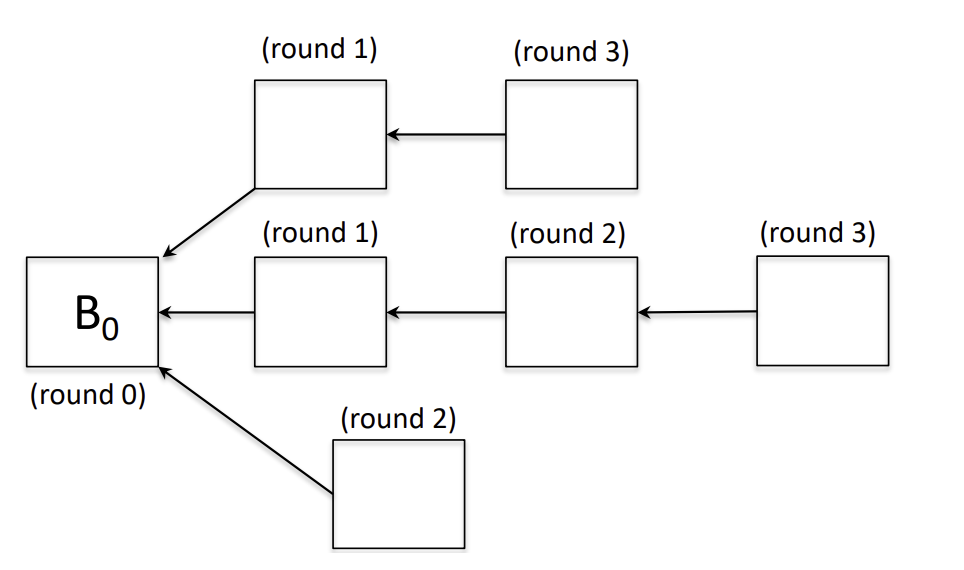
\includegraphics[scale = 0.5]{figures/f23.png}
    \caption{Blocks with round numbers consistent with an assumption (A4): tracing predecessor
pointers back from a block produce a sequence of blocks with strictly decreasing round
numbers.}
    \label{fig:mesh1}
\end{figure}\\

\subsection{Assumptions About Block Production}
The next assumption plays a fundamental role in our analysis of longest-chain consensus
(e.g., in the proofs of Theorem 8.7.1 and 8.9.1), and we’ll need to take care to enforce it in any
concrete implementation.
\nt{\begin{center}
    \textbf{Assumption (A4)}
\end{center}
\noindent
(A4) Every block produced by the round-$r$ leader must claim as its predecessor
some block that belongs to a previous round.}
In other words, if you trace predecessor pointers back from a block, you will encounter a
sequence of blocks with strictly decreasing round numbers (ending in the genesis block, which
we interpret as belonging to round 0). In particular, because this assumption rules out any
cycles among the produced blocks, our visualization of longest-chain consensus as an evergrowing in-tree is accurate. This assumption also automatically rules out the possibility of
two blocks from the same round appearing on a common chain (Figure 8.2).\\
Your first reaction to assumption (A4) might be that it seems obvious—how can a block
refer to something that doesn't exist yet? The assumption rules out two possibilities that
would otherwise be problematic. First, remember that in step (2b) a (Byzantine) node might
create multiple round-$r$ blocks; assumption (A4) makes the non-trivial assertion that none
of these round-$r$ blocks can point to each other as predecessors. (The node can still create a
bunch of round-$r$ blocks, for example using some round-$(r-1)$ block as the predecessor for all
of them.) Second, one possible strategy for a Byzantine node that is selected as the round-$r$
leader is to delay the announcement of its choices in step (2b) until later. (We inevitably
have to deal with this possibility, because it can be indistinguishable from an honest node
that has had its messages delayed.) For example, imagine node 17 is a Byzantine node
selected as the leader of round 117, and only in round 125 does it announce “by the way,
here are my round-117 blocks and their predecessors,” with some of the named predecessors
created only in rounds 118–124. Assumption (A4) asserts that Byzantine nodes should be
unable to get away with this.\\
Assumption (A4) is crucial to our analysis (as will be obvious in Sections 8–11), but
it’s actually pretty trivial to enforce in all three scenarios that we’re thinking about. In
scenario (PKI), for example, the obvious approach is to require that each block proposal
is accompanied by a round number and a signature from the leader of that round, and for
honest nodes to ignore any block proposal in which the round number of the predecessor
block is at least as large as that of the new block. The exact same idea can be used in
scenario (PoS).\\

\noindent
\textbf{A stronger property in the proof-of-work setting.} Scenario (PoW) is the interesting
one, and in fact blocks will not be explicitly annotated with their round number. As we’ll see
in chapter 9, typical proof-of-work-based implementations of longest-chain consensus require
nodes to commit to their choices in step (2b) before they’re even notified that they’re the
round’s leader. (Technically, solutions to cryptographic puzzles are regarded as valid by
honest nodes only if they include an encoding of the node’s step (2b) choices, and validity
can only be checked after the proposed solution has been assembled.) Because they commit
to their block proposals before round $r$ has started (it starts only once they've validated their
winning lottery ticket, including the block proposals encoded by the ticket), those blocks can
only refer to predecessor blocks that exist at that time (which, by definition, were created
in rounds prior to $r$).
Given that, in scenario (PoW), winning lottery tickets by definition must encode the
node’s decisions in step (2b), why not further restrict the ticket format so that the node specifies exactly one (rather than many) round-$r$ block, along with its predecessor? (As we’ll see,
honest nodes are anyways supposed to propose exactly one block in a round of longest-chain
consensus.) By incorporating this idea, typical implementations of longest-chain consensus
in scenario (PoW) wind up enforcing a stronger version of assumption (A4):
\nt{
\begin{center}
    \textbf{Assumption (A4) [Stronger Proof-of-Work Version]}
\end{center}
\noindent
(A4’) The leader of a round produces exactly one block, and this block claims
as its predecessor some block that belongs to a previous round.}
The fundamental consistency and liveness guarantees of longest-chain consensus (Theorems ?? and 10.1) depend only on assumption (A4), not on the stronger version satisfied by
typical proof-of-work instantiations. (Though, as we’ll see, the proof of consistency does get
easier if you can assume (A4’) and not just (A4).) This is exactly the kind of insight that
you miss by studying the Bitcoin protocol for its own sake rather than by examining each
of its ingredients in isolation. This point also demonstrates the value of crisply articulating
the minimal assumptions required for the validity of an argument—as it turns out, many
ideas that were originally developed to analyze the (PoW) scenario specifically can be reused
directly for the other two scenarios as well.

\subsection{Assumptions About Communication}
You should be bothered by our final assumption, which is patently false:

\nt{\begin{center}
    \textbf{Assumption (A5)}
\end{center}
\noindent
(A5) At all times, all honest nodes know about the exact same set of blocks
(and predecessors).}
Alternatively, you can think of assumption (A5) as asserting that we’re working in the
synchronous model with the maximum message delay $\Delta$ equal to zero—whenever, an honest
node learns anything new, it can then instantly communicate (by clairvoyance, in effect) the
new information to all the honest nodes. We’ll sometimes call this the “super-synchronous”
or “instant communication” model (neither of which are standard terms).\\
Even when we work in the synchronous model with $\Delta = 1$, there will be periods of time
in which different honest nodes know different things. For example, when an honest leader
proposes a new block, it knows about that block one time step earlier than the other honest
nodes.\\

\noindent
\textbf{The plan.} Unlike assumption (A1), we can’t take (A5) on faith—it’s simply not true.
Unlike assumptions (A2)–(A4), we can’t design a consensus protocol to enforce it—message
delays are outside the control of the protocol. So what’s the plan and the reasoning behind
it?
\begin{enumerate}
    \item We’ll adopt assumption (A5) temporarily, and will relax it later. (We could relax it
in this chapter, but the most sensible place to do so is in chapter 9, in the context of
scenario (PoW).)
    \item The vast majority of interesting and non-trivial ideas in the analysis of longest-chain
consensus are necessary even under assumption (A5).
    \item These ideas are easier to understand in the safe confines provided by assumption (A5),
unoccluded by other details.
    \item All the guarantees we’ll prove for longest-chain consensus under assumption (A5) will
hold more generally in the traditional synchronous model, provided the maximum message delay $\Delta$ is small relative to the average length of a round.
    \item The analysis of this extension to the synchronous model (discussed in chapter 9) is conceptually straightforward once the main ideas in this chapter (under assumption (A5)) have been properly internalized. (Warning: some amount of math is involved.)
\end{enumerate}

Consistency vs. finality. Still, you’d be right to ask: “Isn’t the whole point of state
machine replication to keep nodes in sync? And haven’t you trivialized the problem by
asserting that all nodes automatically know the same information?” That’s a good criticism.
Assumption (A5) doesn't trivialize liveness, but it does seem to trivialize consistency. But
let’s split “consistency” into two conceptually different properties:\\
\noindent
(i) consistency between different nodes at a given moment in time; and\\
\noindent
(ii) “self-consistency,” meaning consistency between an honest node and a future version
of itself.\\

Property (i) is obviously trivialized by assumption (A5), so let’s look at property (ii).
“Consistency with one’s future self” means if an honest node $i$ regards a block $B$ as
finalized at time $t$, then the block should never be rolled back: node $i$ should regard $B$ as
finalized also at all moments in time after $t$. (The order of finalized blocks should also remain
the same.) We’ll sometimes refer to this property as—wait for it—finality.
In previous chapters, property (ii) was baked into the definition of the SMR problem—
remember that every node maintains an append-only data structure of transactions. (Note
“append-only” is equivalent to “nothing gets rolled back.”) And for BFT-type consensus
protocols like Tendermint, the way we proved consistency for different nodes—by arguing
via quorum certificates that there will never be two different blocks finalized at the same
block height—immediately implies that (assuming $f < \frac{n}{3}$) no honest node would ever roll
back an already-committed block. Longest-chain consensus, however, can be vulnerable to
violations of finality in the form of rollbacks. Even under assumption (A5), it is not at all
trivial to prove that the protocol satisfies such self-consistency under reasonable assumptions.
And happily, the main ideas that prove finality (ii) under assumption (A5) (in Theorem 8.8.1)
can be largely reused to also prove consistency between nodes (i) when assumption (A5) is
relaxed (to the traditional synchronous model, with a parameter $\Delta$ that is small relative to
the average round length).\\

\subsection{Recap}
Here are the five assumptions, collected together for convenience:
\nt{
\begin{center}
    \textbf{Assumptions (A1)–(A5)}
\end{center}
\noindent
(A1) No node knows the genesis block prior to the deployment of
the protocol.\\
\noindent
(A2) It is easy for all nodes to verify whether a given node is the leader of a
given round.\\
\noindent
(A3) No node can influence the probability with which it is selected as the
leader of a round in step (2a).\\
\noindent
(A4) Every block produced by the round-$r$ leader must claim as its predecessor
some block that belongs to a previous round.\\
\noindent
(A5) At all times, all honest nodes know about the same set of blocks
(and predecessors).}
You should be wondering about the roles of these assumptions in this chapter’s analysis. The
analysis will be modular, with two main steps. One step identifies a sufficient condition on the
sequence of leaders chosen in step (2a) of longest-chain consensus—a type of “balancedness
property”—under which the protocol satisfies consistency and liveness (see Section 8–11).
The other step (see Section 8.6) identifies conditions (on the amount of Byzantine participation and the method of leader selection, e.g. random leader selection) that guarantee the
generation of a balanced leader sequence (perhaps with high probability). Assumptions (A2)
and (A3) are about the integrity of the leader selection process; accordingly, they show up
(somewhat implicitly) in Section 8.6, as part of proving that Byzantine leaders will not be
overly frequent.\\
The other three assumptions are all important for ruling out the possibility that infrequent Byzantine leaders can cause an outsized amount of havoc on the protocol. The role of
assumption (A1) is a bit subtle, while assumptions (A4) and (A5) will be crucial
to the analysis. I think it will also be intuitively clear from this chapter’s analysis that assumption (A5) is overkill and that similar arguments should work (perhaps with a slightly
messier proof) in the general synchronous model (with delay parameter $\Delta$ well less than the
typical round length). Here’s a table summarizing the roles of the five assumptions:
\begin{center}
\begin{tabular}{ | m{2.5cm} | m{2.5cm}| m{4cm} | } 
  \hline
  Assumption & Type & Used in Which Proofs? \\ 
  \hline
  (A1) & trusted setup & Theorem 8.7.1 \\ 
  \hline
  (A2) & to be enforced  & implicit in Section 8.6 \\ 
  \hline
  (A3) & to be enforced  & implicit in Section 8.6 \\ 
  \hline
  (A4) & to be enforced  & Theorems 8.7.1, 8.9.1, and 8.10.1 \\ 
  \hline
  (A5) & to be relaxed & Theorems 8.7.1, 8.9.1, and 8.10.1 \\ 
  \hline
\end{tabular}
\end{center}

\begin{figure}[h]
    \centering
    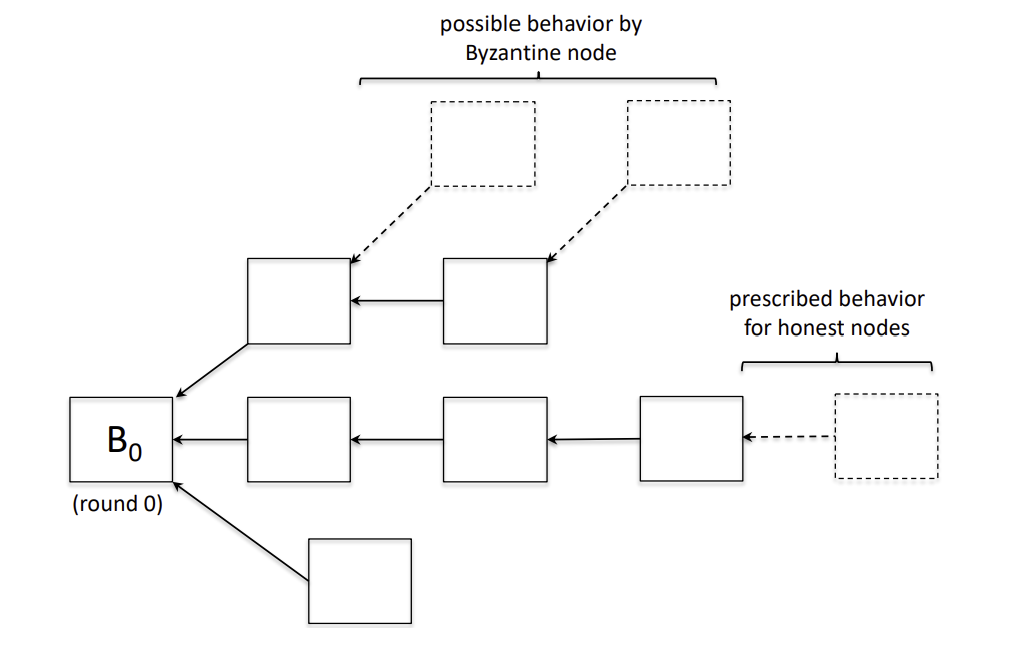
\includegraphics[scale = 0.5]{figures/f24.png}
    \caption{Honest nodes are instructed to propose a single block that extends the longest
chain (with ties broken arbitrarily). Byzantine nodes might propose multiple blocks, and
might name predecessors other than the end of the longest chain.
}
    \label{fig:mesh1}
\end{figure}\\

\section{Honest vs. Dishonest Behavior}
\subsection{Prescribed Behavior for Honest Nodes}
Now that we understand what longest-chain consensus looks like at a high-level, let’s discuss
what honest nodes are supposed to do (in step (2b), once selected as a leader) and how
Byzantine nodes might deviate from that prescribed behavior.\\

\noindent
\textbf{Honest blocks include all transactions.} First, when selected as a leader, an honest
node assembles a block from scratch as in our previous SMR protocols—by including all
the as-yet-unexecuted transactions that it knows about (perhaps directly from a client, or
perhaps from another node), in some arbitrary order. Note that an honest node proposes
exactly one block each time it’s selected as the leader of a round.\\

\noindent
\textbf{Extend the longest chain.} What about the predecessor? An honest leader is instructed
to look over the in-tree of all the blocks that it knows about and set its block’s predecessor to
the existing block that is furthest (in terms of number of hops) from the root (i.e., from the
genesis block). In other words, an honest node adds its block to the end of the longest chain,
making that chain still longer (Figure 8.3). And what if there’s a tie, with two or more equally
long chains? For our consistency and liveness analysis, we’ll be pessimistic
and assume that honest nodes break ties in an arbitrary (e.g., adversarially chosen) manner.
You could imagine imposing a tie-breaking rule that honest nodes are supposed to follow
(e.g., randomly, or in favor of the block heard about earlier), but guarantees as important
as consistency and liveness should not be so fragile as to hinge on how honest nodes carry
out tie-breaking.\\

\noindent
\textbf{Immediate announcements.} Finally—this may seem obvious, but it is something that
Byzantine nodes might deviate from—honest nodes are expected to broadcast their chosen
block and predecessor immediately after they discover that they’re the leader of the current
round.
\subsevtion{Deviations by Byzantine Nodes}
A Byzantine node might deviate from the three instructions above in arbitrary ways—
proposing more than one block or a block that doesn't contain all known transactions (or
even an empty block), naming as a predecessor a block other than the end of the longest
chain, and delaying the announcement of block proposals until some later point in time.\\

\noindent
\textbf{Empty blocks.} The first type of deviation doesn't seem that bad—we've had to deal with
the threat of Byzantine leaders proposing dishonest blocks ever since the SMR protocol based
on iterating the Dolev-Strong protocol back in Chapter 2. Unlike in Chapter 2, however, there
is no guarantee that any given honestly proposed block will eventually get finalized. Our
liveness analysis in Section 8.9 will have to address this issue by arguing that honest nodes
regularly manage to assemble blocks that eventually get finalized (if all finalized blocks came
from Byzantine block proposers, they might all be empty in which case all transactions would
be starved).\\

\noindent
\textbf{Delayed block announcements.} For the consistency and liveness analysis in this chapter, the third type of deviation (delayed block announcements) turns out not
to matter (other than making the proofs more annoying). Looking ahead, it will matter in
Chapter 10 when we study the case of block producers competing for “block rewards.” (As
we’ll see, this also relates to the “chain quality” discussion in Section 8.10.) We’ll see in that
chapter that, perhaps counterintuitively, there are scenarios in which a node can increase
its block rewards (relative to honestly following the protocol) via a deviation that includes
strategically delayed block announcements.\\

\noindent
\textbf{Deliberate forking.} Deviations of the second type—the deliberate creation or perpetuation of forks through the extension of blocks other than the end of the longest chain—should
be immediately worrying, and they will be the focus of this Chapter’s analysis. Why are they
worrying? Honest nodes are effectively trying to coordinate on a single (longest) chain, and
absent interference by Byzantine nodes the longest chain would keep growing longer and
longer. A block that does not extend the longest chain, not only fails to make the longest
chain longer, but also threatens to switch which chain is the longest, which would lead to a
rollback of blocks on the previously longest chain.\\
For example, suppose there are 10 rounds in a row with Byzantine leaders. These Byzantine nodes can collaborate and grow a fork of length 10 starting from 9 blocks back, to roll
back the last 9 blocks of what had been the longest chain (Figure 8.4). More generally, a
sequence of $k$ consecutive Byzantine leaders is in a position to roll back $k - 1$ blocks. Still more generally, if there is a sequence of leaders in which the Byzantine leaders outnumber
the honest leaders by $k$, the Byzantine nodes can roll back the last $k - 1$ blocks of what had
been the longest chain (why?). For example, if in a window of 1000 rounds, there are 510
Byzantine leaders and 490 honest leaders, the Byzantine nodes are in a position to roll back
the last 19 blocks of what was the longest chain at the start of the window. (In fact, under
our assumption of worst-case tie-breaking by honest nodes, such a set of Byzantine nodes
could even roll back $k$ blocks.)\\
\begin{figure}[h]
    \centering
    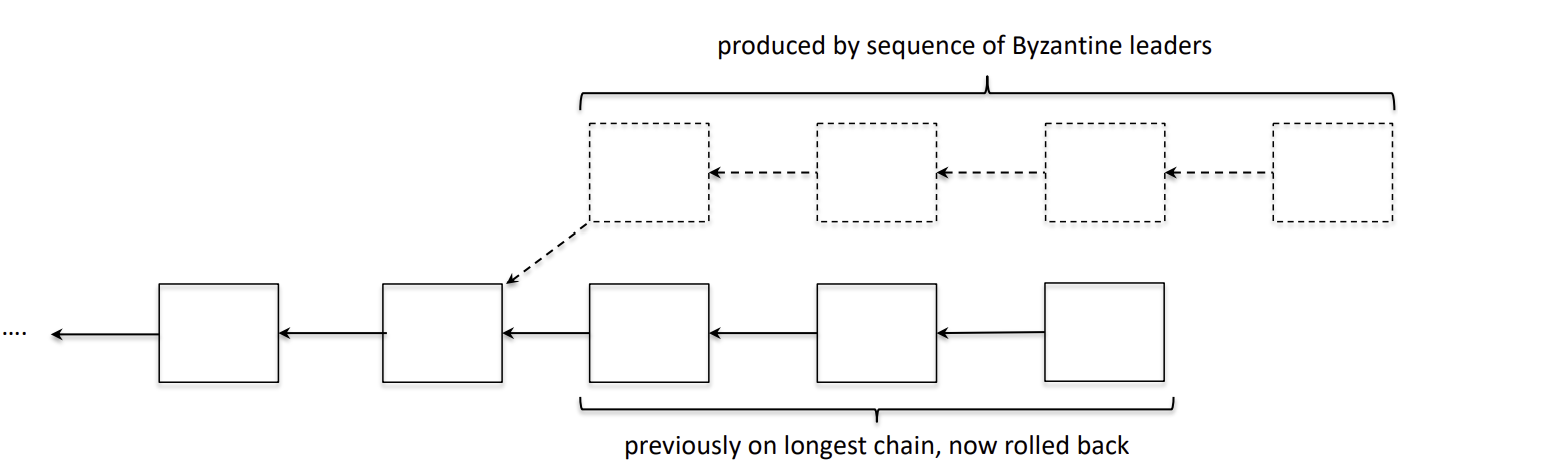
\includegraphics[scale = 0.5]{figures/f25.png}
    \caption{ A sequence of $k$ consecutive Byzantine leaders are in a position to roll back $k − 1$
blocks. (Or even, with worst-case tie-breaking by honest nodes, $k$ blocks.)}
    \label{fig:mesh1}
\end{figure}\\
\noindent
\textbf{Takeaways.} What can we learn from these examples of deliberate forking? Three things:
\begin{enumerate}
    \item With longest-chain consensus, you should always regard the last several blocks of
the longest chain as tentative—not-yet-finalized and still under negotiation. In other
words, a block should be considered finalized only once it is ensconced sufficiently
deeply on the longest chain, already extended by several other blocks. How deep
on the longest chain does the block need to be before it can be safely considered finalized? That’s an important question, which we’ll start tackling head-on in the next
section.
    \item The examples above point out a fundamental obstruction to proving any kind of finality
result for longest-chain consensus: if you can’t rule out sequences of leaders in which
the number of Byzantine leaders outnumbers the number of honest leaders by $k$, then
you can’t expect any kind of finality to hold for any of the last $k - 1$ (or even $k$)
blocks on the longest chain. The best-case scenario would be that this is the only
obstruction, meaning that the converse also holds: if you can rule out such windows,
then finality does hold for all the blocks on the longest chain other than the last $k$
of them. This converse constitutes the essence of our forthcoming analysis of the
consistency of longest-chain consensus.
    \item This style of deliberate forking shows that there’s no hope of proving anything about
longest-chain consensus unless strictly less than half of the nodes are Byzantine. To
see this, imagine that 51\% of the nodes are Byzantine. Assume that leader selection is
done in a way that every node gets its fair share of turns. Then, 51\% of the rounds
will have Byzantine leaders. In a window of 1000 consecutive leaders you’re likely to
see something like 510 Byzantine nodes and 490 honest nodes, and these Byzantine
nodes are then in a position to roll back the last 20 blocks of the once-longest chain. In
a window of 10000 nodes, if there are 5100 Byzantine leaders and 4900 honest leaders,
the Byzantine nodes will be able to roll back the last 200 blocks of the once-longest
chain. And so on. Given that Byzantine leaders can outnumber honest leaders by an
arbitrarily large amount (as the sequence length grows large), no block is ever safe
from being rolled back—the Byzantine nodes effectively have dictatorial control over
which blocks wind up on the longest chain.
So, a necessary condition for the longest-chain consensus to have any provable guarantees
is that more than half of the nodes run the protocol honestly and correctly; the best-case scenario would be that this condition is also sufficient (for provable consistency
and liveness). Great news: this is exactly what we’ll prove!
\end{enumerate}

\section{Which Blocks Are Finalized?}
Given the power of the potential deviations (specifically, deliberate forking) by Byzantine
nodes identified in the previous section, we've homed in on the coolest statement that might
conceivably be true about longest-chain consensus: that whenever more than 50% of the
nodes running the protocol are honest, all blocks on the longest chain other than the last k
can be considered finalized. (Along with the other usual desired properties, like liveness.)
And this is exactly the main punchline of the analysis in this chapter.
\subsection{The Parameter $k$}
The parameter $k$-the number of blocks at the end of the longest chain that are still considered unfinalized and under negotiation—will obviously be an important one for us. On the
one hand, we’d like it to be as small as possible (so that blocks of transactions get finalized as
soon as possible after they are created); on the other, intuitively, larger (more conservative)
values of $k$ seem more likely to allow for provable consistency guarantees.
Let’s introduce some notation to reason about this parameter: for an in-tree $G$ of blocks
(rooted at the genesis block) and a nonnegative integer $k$, define:
$$B_k(G) := \text{the longest chain of $G$, with the last $k$ blocks removed.} \quad(1)$$
For example, for the in-tree $G$ in Figure 8.5, $B_2(G)$ is the chain $B_0 \gets B_2 \gets B_4$ while $B_3(G)$
is the chain $B_0 \gets B_2$.
There are two possible points of confusion about this definition.\\
\begin{figure}[h]
    \centering
    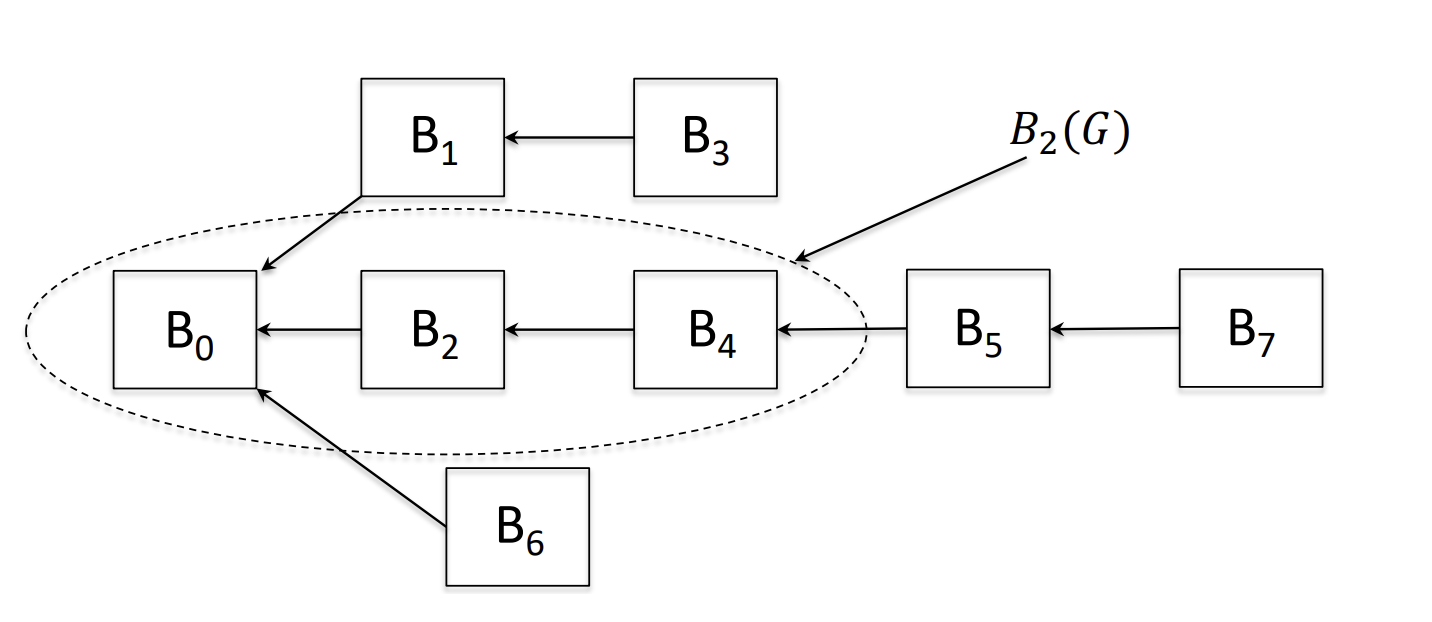
\includegraphics[scale = 0.5]{figures/f26.png}
    \caption{$B_k(G)$ denotes the longest chain of the in-tree $G$, with the last $k$ blocks removed
}
    \label{fig:mesh1}
\end{figure}\\

Defined client-side rather than in-protocol. If you look at the description of longestchain consensus in Section 8.2, you’ll notice that there’s no parameter $k$—the evolution of the protocol is completely independent of what value of $k$ you might have in mind. Rather, the
parameter $k$ dictates how to interpret the evolution of the protocol—how many blocks at
the end of the longest chain you should regard as “still tentative” in some sense.
The parameter $k$ is in the eye of the beholder, and can therefore be set client-side, and
differently for different clients. (We’re using “client” here in the usual tech sense—the userfacing application that interacts with the blockchain—rather than in the strict SMR sense.)
For example, imagine a blockchain protocol based on longest-chain consensus that also has
a native currency (like Bitcoin), and imagine that you’re a seller who accepts payments in
this currency. If you’re a high-volume seller of a low-cost product, like cups of coffee, you
might be content to hand over a cup of coffee to a customer after that customer’s payment
transaction has been added to the longest chain and extended by a single block ($k = 1$).
You’d run some risk of the transaction getting rolled back (and the customer effectively
getting a free cup of coffee), but perhaps you view minimizing customer wait time as more
important. If you’re selling Teslas, on the other hand, probably you want to make the
customer wait for awhile (maybe $k = 100$), so that you can be confident that their payment
can be regarded as finalized, never to be evicted from the longest chain.
Is $B_k(G)$ well defined? The second point of confusion, which you’d be right to wonder
about, is whether the notation $B_k(G)$ is even well defined in a mathematical sense. In (1),
who am I to write “the longest chain,” when we all know that there might be multiple chains
tied for the longest? Figure 8.6 depicts an in-tree $G$ with two longest chains. Here, $B_2(G)$
actually is well defined—no matter which of the two longest chains you choose, after lopping
off the last two blocks, you get the same thing (the chain $B_0 \gets B_2$). But $B_1(G)$ is not well
defined, because if you lop off only one block from the end, you’re still left with different chains
($B_0 \gets B_2 \gets B_4$ and $B_0 \gets B_2 \gets B_5$). In general, when we say that “$B_k(G)$ is well defined,”
we mean that it doesn't matter which longest chain you choose, after lopping off the last $k$
blocks you get the same thing. Equivalently, all longest chains agree on all their blocks
except possibly for their last $k$. Said still another way, all longest chains share a common
prefix—if they all have length $l$, then the prefix of the first $l - k$ blocks is shared across
them.

\begin{figure}[h]
    \centering
    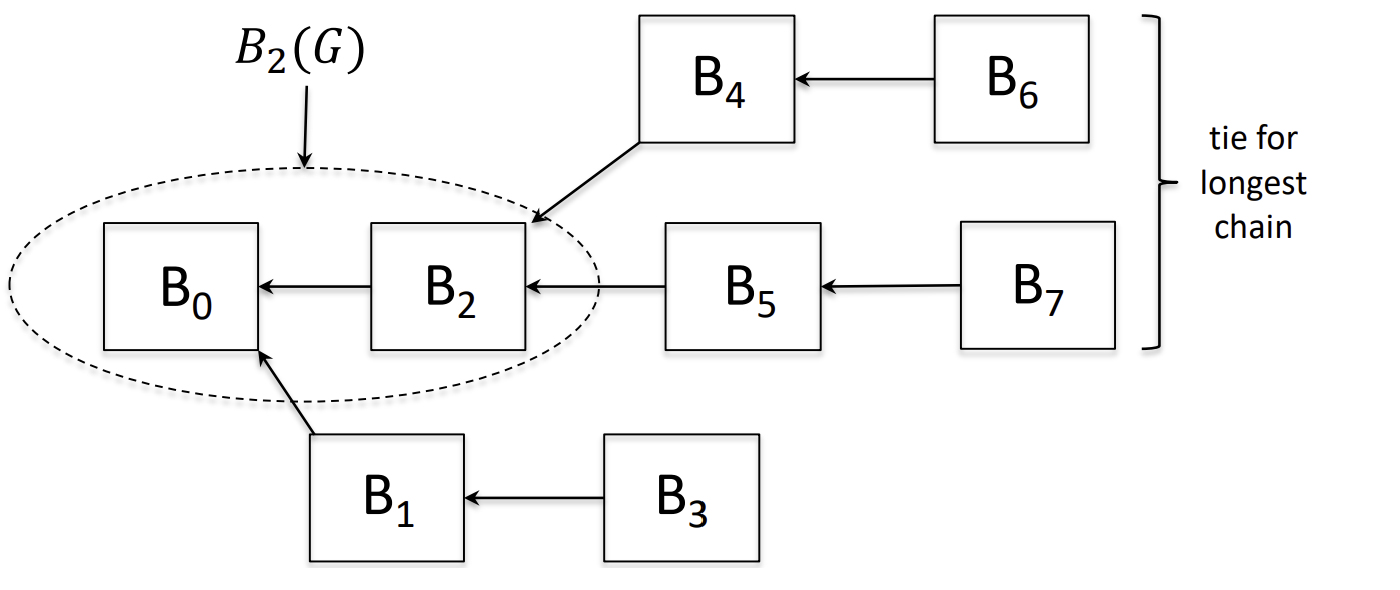
\includegraphics[scale = 0.5]{figures/f27.png}
    \caption{ When there is a tie for the longest chain, $B_k(G)$ may or may not be well defined.
}
    \label{fig:mesh1}
\end{figure}\\

\subsection{Balanced Leader Sequences}
In our analysis, the first order of business (Theorem 8.7.1) will be to prove this “common prefix
property”: provided more than 50\% of the nodes are honest and $k$ is sufficiently large (and
under our standing assumptions (A1)–(A5)), $B_k(G)$ is guaranteed to be well defined. From
there, the goal will be to prove finality, meaning that the blocks of $B_k(G)$ can be considered
finalized (Theorem 8.8.1), and liveness, meaning that $B_k(G)$ continues to grow over time, with
blocks assembled by honest nodes regularly added (Theorem 8.9.1).\\

\noindent
\textbf{The plan.} Our analysis will be modular. To explain, consider a sequence of rounds of
longest-chain consensus and their corresponding leaders. If you think about it, there’s no
need to differentiate between which honest node is selected as a leader (each is following the
protocol and thus behaving identically) nor which Byzantine node is selected as a leader (we
always assume that Byzantine nodes are acting in cahoots, so it doesn't matter which one
is chosen). We can therefore think of the leaders of a sequence of rounds as a bunch of “H”s
(for honest) and “A”s (for adversarial). For example, we argued in the previous section that
in any sequence of rounds in which there are $k$ more “A”s than “H”s, the Byzantine nodes
are in a position to cancel the last $k$ blocks of the current longest chain. The plan for the
modular analysis is then:
\begin{enumerate}
    \item (Definition 8.5.1) State a definition that articulates a condition that a given leader sequence may or may not meet.
    \item (Sections 8.7–8.10) Prove that, as long as the sequence of leaders generated in longestchain consensus satisfies this condition (and the parameter $k$ is chosen appropriately,
and assumptions (A1)–(A5) hold), the protocol satisfies all the properties that we want
(consistency, liveness, etc.).
    \item (Section 8.6) Prove that, as long as more than half of the nodes running the protocol are
honest, this condition is satisfied (perhaps with high probability).
\end{enumerate}
Chaining together the second and third steps shows exactly what we want: as long as
more than half the nodes are honest and the parameter $k$ is set appropriately, longest-chain
consensus enjoys provable consistency and liveness guarantees.\\

\noindent
\textbf{Balanced leader sequences.} Here’s the key definition (with respect to a parameter w,
which stands for “window” and is a positive integer):
\dfn{$w$-Balanced Leader Sequence}{A sequence $_1, l_2, l_3, \cdots \in \{H, A\}$ is wbalanced if, in every window $l_i
, l_i+1, \cdots , l_j-1, l_j$ of length at least $w$, the $H$’s outnumber the $A$’s.}

The bigger $w$ is, the easier Definition 8.5.1 is to satisfy (because there are fewer windows to
worry about). Thus we will generally be interested in the smallest $w$ for which a leader
sequence is $w$-balanced.\\
For example, any leader sequence that includes at least one Byzantine node fails to be
1- or 2-balanced (in a window of length 1 or 2 that contains that node, the honest nodes do
not outnumber the Byzantine nodes). A sequence in which every pair of Byzantine leaders
are separated by at least two honest nodes is 3-balanced (why?). A sequence generated by
the round-robin rotation through $n$ nodes, with $f < \frac{n}{3}$ Byzantine nodes, is n-balanced
(why?). (Homework: what about with the weaker condition $f < \frac{n}{2}$?) A leader sequence
in which the average frequency of Byzantine nodes exceeds that of honest nodes—e.g., with
$f > \frac{n}{2}$ and either round-robin or random leader selection—will not be w-balanced for
any $w$ (why?).\\

\noindent
\textbf{Implementing the second step of the plan.} Let’s connect Definition 8.5.1 back to the
second takeaway from Section 8.4. We saw in that section how, in a window in which there
are $k$ more Byzantine nodes than honest nodes, Byzantine nodes can cancel the last $k$ blocks
of the current longest chain. The best-case scenario is that this obstruction to finality is
the only obstruction to finality, meaning that as long as there are no windows in which the
number of Byzantine nodes outnumber the honest nodes by more than $k$, all but the last k
blocks of the longest chain can safely be considered finalized.
In a w-balanced leader sequence, meanwhile, there cannot be any window in which the
Byzantine nodes outnumber the honest nodes by $\frac{w}{2}$ or more (why?). The dream, then,
would be that whenever Definition 6.1 is satisfied with some parameter $w$, all but the last
$\frac{w}{2} - 1$ blocks of the longest chain can be considered finalized. And this is exactly what we’re going to prove in Theorem 8.8.1 (under the assumptions (A1)–(A5) from Section 8.3)!
Specifically, in Section 8.7 we’ll use the $w$-balancedness condition to establish the common
prefix property (Theorem 8.7.1)—i.e., that the notation $B_k(G)$ above is well defined, with all
longest chains agreeing on all but possibly their final $k$ blocks. The finality guarantee
in Theorem 8.8.1 then follows easily in Section 8.8. We’ll also use the w-balanced condition
in the proofs of liveness (Theorem 8.9.1 in Section 8.9) and chain quality (Theorem 8.7.10.2 in
Section 8.10).\\

\noindent
\textbf{Implementing the third step.} The second step of our modular analysis shows that if
your leader sequence is balanced—for whatever reason—then you’re good, with all the consistency and liveness properties that you might want.
But why should the leader sequence be balanced in the first place? We already argued that it
won’t be balanced if more than half the nodes are Byzantine, but why should it be balanced
if more than half the nodes are honest?\\
In Section 8.6 we’ll drill down on the version of longest-chain consensus in which each
leader is chosen independently and uniformly at random. (This is a natural design already
in scenario (PKI), but more importantly it’s completely essential to the permissionless implementations of longest-chain consensus in chapters 9 and 12 for scenarios (PoW) and (PoS),
respectively.) The punchline of the analysis in Section 8.6 will be that, as long as less than half
the nodes are Byzantine, random leader selection generates a balanced leader sequence with
high probability. The intuition is that—by the law of large numbers, essentially—honest
nodes will have (almost) proportional representation in every sufficiently large window of
consecutive leaders. (E.g., if 51\% of the nodes are honest, then in all sufficiently large
windows there should be somewhere between 50.5\% and 51.5\% honest nodes.)\\
How balanced a sequence, exactly—how big do the window lengths need to be before
proportional representation kicks in? (Remember that the more balanced the leader sequence
is—i.e., the smaller $w$ is—the smaller we can take $k$ and the faster blocks can be finalized.)
The answer depends on various parameters (the fraction of nodes that are Byzantine, the
duration you’re interested in, and the acceptable failure probability), and we’ll get into the
details in the next section. For typical parameter values, the analysis suggests taking $k$ (the
number of additional blocks needed before considering a block to be final) in the low-to-mid
double-digits. More aggressive values are often used in practice—for example, for the Bitcoin protocol the famous rule of thumb is to take $k = 6$. (Though when selling a Tesla, $k$ should definitely be taken to something larger than that!)

\section{Random Leaders Are Balanced}

\subsection{Random Leaders and Probabilistic Guarantees}
We’ll see in the next few sections proofs that, as long as the sequence of leaders generated in
longest-chain consensus is w-balanced (see Definition 8.5.1), the protocol satisfies consistency
and liveness (with the parameter $k$ chosen appropriately). When can we count on a balanced sequence of leaders? And for what balance
parameter $w$?\\
In this section we’ll investigate, in scenario (PKI), the version of longest-chain consensus
in which, every round, the leader is selected uniformly at random from the set of all nodes
(i.e., with each node equally likely to be chosen). This is a natural approach to take in the
permissioned setting, but it also extends amazingly gracefully to the permissionless setting
(scenarios (PoW) and (PoW), see chapters 9 and 12).\\
Even in the permissioned setting, given that we want a balanced leader sequence, random
leaders sound like a pretty good idea. For example, imagine that there are 3000 nodes, 1000
of which are Byzantine. If we cycle through the nodes in some fixed round-robin order,
for all we know all 1000 Byzantine nodes appear consecutively in the ordering. In this
case, the leader sequence generated is 2001-balanced but not w-balanced for any $w < 2001$
(why?). If instead each leader is selected randomly, then any given leader has a two-out-ofthree chance of being honest. You might of course get a few Byzantine leaders in a row by
random chance, but getting something like 100 Byzantine leaders in a row—an event with
probability (1/3)100—would presumably happen so rarely that we could ignore the possibility.\\

\noindent
\textbf{Probabilistic finality and liveness.} On the other hand, no matter how big $w$ is, there is
some positive—if astronomically small—probability of seeing $w$ Byzantine leaders in a row.
And this would be true even if there was only one Byzantine node! Thus with randomly
selected leaders, there’s no hope of proving any guarantees for longest-chain consensus that
hold with certainty. (For example, any block might eventually get rolled back if the protocol
winds up choosing a sufficiently long sequence of consecutive Byzantine leaders.) The bestcase scenario would be to prove that consistency and liveness hold with high probability
(meaning probability close to 1, like 99.9\%). Such probabilistic guarantees are typical of
permissionless implementations of longest-chain consensus (including Bitcoin). If the failure
probability is sufficiently small (e.g., less than the probability of your neighborhood getting
hit by an asteroid in the next 24 hours), then probabilistic guarantees are for all practical
purposes as good as deterministic guarantees.

\subsection{Intuition for the Analysis}
Taking the second step of this chapter’s analysis (Section 8.7–8.10)—that a balanced leader
sequence gives you strong consistency and liveness guarantees—on faith for now, let’s investigate the extent to which a sequence of random leaders is balanced. We’ll keep the discussion
a bit on the intuitive and informal side; it wouldn't be hard to turn this discussion into 
rigorous proof, but that wouldn't be the best use of our time.
Let $\alpha$ denote the fraction of nodes that are Byzantine (in terms of our usual notation,
$\alpha = \frac{f}{n}$). We saw in Section 8.4 that there’s no hope of proving anything unless $\alpha < \frac{1}{2}$, so
let’s go ahead and assume that from here on out. The basic idea is:
\begin{enumerate}
    \item A consequence of the law of large numbers is the hopefully intuitive fact that if you
repeat an experiment with success probability $p$ a large number of times, the long-run
fraction of successes you’ll see is almost always going to be roughly $p$.
    \item Identifying a successful experiment with the selection of an honest leader, means
that after enough repeated trials the long-run fraction of honest leaders is almost always
going to be roughly $1 - \alpha$.
    \item Because $\alpha < \frac{1}{2}$, this proportional representation of honest leaders means that the honest
leaders should outnumber the Byzantine leaders in every sufficiently large window.
\end{enumerate}
The parameter $w$ in the $w$-balancedness condition will control how large we need to take
the parameter $k$—the number of subsequent blocks required to regard a block as finalized—
to guarantee consistency and liveness. Time-to-finalization is an important performance
characteristic of a blockchain protocol, so we’d like a more quantitative understanding of
just how balanced a sequence of random leaders is likely to be.\\


\noindent\textbf{Toward a quantitative understanding}. The exact guarantee on the parameter $w$ will
depend on just how far $\alpha$ is from $\frac{1}{2}$—the closer it is to $\alpha$, the bigger the $w$ we’ll need to take
to ensure sufficiently proportional representation of honest leaders.\\
For example, imagine that $\alpha$ is 49\%. In a length-100 window of consecutive leaders, we
would expect 51 honest nodes and 49 Byzantine nodes. There will be some variance, of
course—sometimes there will be 55 honest leaders, sometimes there will be 47 (which would
violate 100-balancedness), and so on. So we would not expect a random leader sequence to
be 100-balanced when $\alpha = 0.49$.\\
In a length-1000 window, meanwhile, we would expect 510 honest nodes and 490 Byzantine nodes—now we have a margin of error of 20 between the two, and it intuitively seems
that we should have a better shot at seeing a majority of honest nodes. Sometimes there
might be 515 honest nodes, sometimes 505, sometimes 523, and sometimes 497 (which would violate
1000-balancedness), and so on. So we might expect a random leader sequence to be 1000-
balanced with somewhat high (but not 99.9\%) probability. Similarly, with length-10000
Windows, we have a buffer of 200 between the expected number of honest and Byzantine
nodes to absorb the inevitable variations, and it would seem still more unlikely to have an
unluckily low number (< 5001) of honest nodes. If this intuition is correct, given a desired failure probability $\delta$, we should be able to take the window length large enough (as a function
of $\alpha$ and $\delta$) to guarantee a failure probability of at most $\delta$.

\subsection{Quantitative Analysis of Random Leader Selection}
Exponentially small bounds. The intuition above is quite accurate. But if you really
want some concrete numbers, you have to do some actual math. And if you do the math,
the very cool thing that you discover is that not only is the probability of a $w$-balancedness
violation decreasing with the window size, it’s decreasing exponentially quickly. More formally:
$$\textbf{Pr}[\text{a given length-w window is at least half Byzantine}] \leq e^{-cw}, \quad(2)$$
where $c$ is some constant (independent of $w$). (The constant $c$ depends on $\alpha$—the closer $\alpha$
is to $\frac{1}{2}$ , the smaller the $c$ and the slower the decrease in failure probability.) If you want to
keep a concrete number in mind, think of $c$ as being (for example) 0.1. Also, the “$e$” in (2)
denotes the base of the natural logarithm, $2.718 \cdots$.\\
An exponentially small failure probability like the one in (2) is good news: every time you
bump up the window length $w$ by 1, the failure probability drops by another constant factor.
This is the key property behind the assertion that random leader sequences are w-balanced
for reasonably small values of $w$ (with high probability). (Remember, $w$ controls the time
to finality, and we want to take it to be as small as possible!)\\

\noindent
\textbf{Applying the Union Bound.} The failure probability in (2) concerns a specific window
(e.g., the leaders of rounds $101, 102, \cdots, 140$). Looking back at Definition 8.5.1, we see that
it asserts something about every window of sufficiently large length (e.g., at least 40 leaders
in a row), not just one window. To bridge that gap, we can use the Union Bound, which
states that the probability that any bad event happens is at most the sum of their individual
probabilities:
$$\textbf{Pr}[\text{at least one of the events $E_1, E_2, \cdots, E_k$ occur}] \leq \sum_{i=1}^k \textbf{Pr}[\text{event $E_i$ occurs}]$$
Or, in terms of the complementary event:
$$\textbf{Pr}[\text{none of the events $E_1, E_2, \cdots, E_k$ occur}] \geq 1 - \sum_{i=1}^k \textbf{Pr}[\text{event $E_i$ occurs}] \quad(3)$$
For us, the individual events $E_i$ correspond to the windows of length at least $w$ (with $E_i$
occurring if and only if the corresponding window is at least half Byzantine leaders). The key point is that, by definition, a leader sequence is w-balanced if and only if none of these
events occur.\\
\begin{figure}[h]
    \centering
    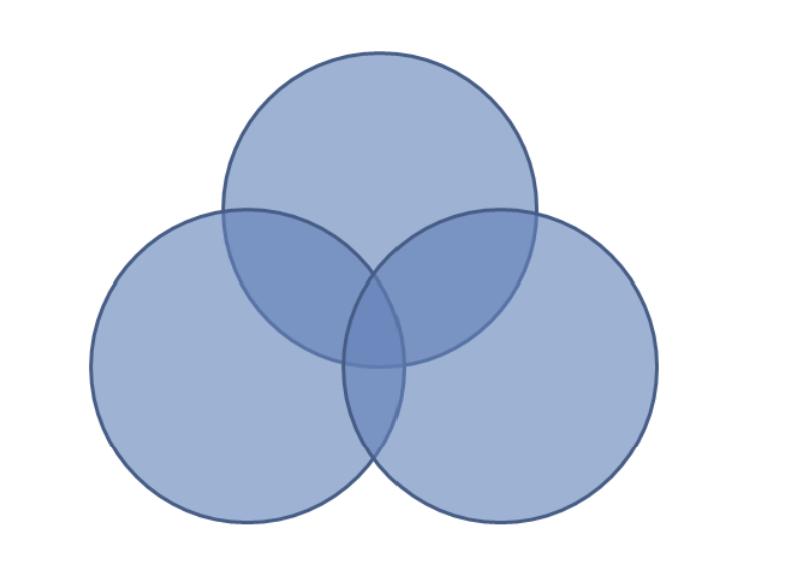
\includegraphics[scale = 0.5]{figures/f28.png}
    \caption{ The Union Bound: the probability of the union of a bunch of events is bounded
above by the sum of the probabilities of the individual events.
}
    \label{fig:mesh1}
\end{figure}\\

Now imagine that we’re interested in some stretch of $T$ consecutive rounds of the longest chain consensus (which could represent a day, a month, etc.). The number of windows (of
length at least $w$, or otherwise) can be bounded above crudely by $T^2$ (with only $T$ choices
for the first and for the last round of the window). Because there are at most $T^2$ $E_i$’s and
(by (2)) $\textbf{Pr}[E_i] \leq e^{-cw}$ for every $i$, the Union Bound (3) tells us that
$$\textbf{Pr}[\text{a sequence of $T$ randomly selected leaders is $w$-balanced}] \geq 1 - T^2. e^{-cw} \quad(4)$$
Solving for $w$ given choices of $T$ and $\delta$ (and $\alpha$). So, is the right-hand side of (4) big
or small? The answer depends on our choice of w. Fix a failure probability $\delta$ that we’re
comfortable with, such as $\delta = 0.01$. The bound in (4) then tells us how to set $w$, by setting
$\delta = T^2 . e^{-cw}$ and then solving for $w$ (by taking logarithms of both sides and rearranging).
When the dust settles, the punchline is:
\nt{a sequence of $T$ random leaders is $w$-balanced with probability at least $1 - \delta$,
provided
$$w \geq c_2(\ln T + \ln \frac{1}{\delta})$$
}
Here, $c_2$ is a constant independent of $w$ and $\delta$. (Like $c_1$, it does depend on $\alpha$—the closer $\alpha$
is to $\frac{1}{2}$, the bigger the constant factor $c_2$.)
The exponentially small probability in (2) thus translates to a lower bound on $w$ that
involves only the logarithms of the two key parameters, the duration T of interest and the
(reciprocal of the) acceptable failure probability. The most important fact about logarithms
is that they grow really slowly—for example, if we’re talking about the base-2 logarithm, the
logarithm of 1000 is roughly 10, the log of one million is roughly 20, the log of one billion
is roughly 30, and so on. This means that we can take the duration T to be quite long and
the failure probability $\delta$ quite small while still getting away with palatable values of $w$.


\noindent\textbf{Recap.}
\begin{enumerate}
    \item As we’ll see in Sections 8.7–8.10, the distance $k$ of a block from the end of the longest
the chain that is required before the block should be considered finalized is controlled by
the smallest w for which the generated leader sequence is $w$-balanced.
    \item Randomly chosen leaders are $w$-balanced with high probability, where the parameter $w$
depends on the fraction $\alpha$ of Byzantine nodes, the duration T of interest, and the
desired failure probability $\delta$ (with $w$ increasing with $\alpha$, $T$, and $\frac{1}{\delta}$).
    \item Because the lower bound on $w$ increases only logarithmically quickly with $T$ and $\frac{1}{\delta}$,
for typical parameter values (say $\alpha = 0.33$, $T = 1000$, and $\delta = .01$) it’s safe to take $w$
(and hence $k$) in the double digits. (A more detailed analysis can be used to improve
this conservative lower bound by a constant factor.)
\end{enumerate}

\subsection{Toward Permissionless Consensus}
Longest-chain consensus is already interesting to study in the permissioned setting (scenario (PKI)), but what’s really special about it is how easily it extends to the permissionless
case. Looking ahead to chapters 9 and 12, let’s examine exactly how the permissioned
assumption was used in the analysis of this section.
Rereading the informal argument in Section 8.6.2, we see that only one thing matters for
the analysis: every round, the probability that a Byzantine node is selected as the leader
is less than 50\%. (This then leads to (almost) proportional representation of honest nodes in
sufficiently long windows, all of which will then have a majority of honest nodes.)
\nt{\begin{center}
    \textbf{Key Property for Analysis of Random Leaders}
\end{center}
There is a constant $\alpha < \frac{1}{2}$
such that, in every round, the probability that a
Byzantine node is selected as the round’s leader is at most $\alpha$. (Also, each
leader should be chosen independently of any of the previous ones.)}

If this key property holds—for whatever reason, whatever the concrete implementation of
longest-chain consensus—the “proportional representation” argument remains valid.21
Now, in scenario (PKI), it’s easy to think of a combination of assumptions and protocol
design choices that together ensure that the key property above holds: if less than half the
nodes are Byzantine and each leader is selected independently and uniformly at random from
the set of all nodes, then the probability that a given round has a Byzantine leader is less
than 50\%.\\
In the permissionless scenarios (PoW) and (PoS), where the set of nodes running the
protocol is unknown, it’s not obvious how to sample a node uniformly at random. But, if we can find a combination of assumptions and (permissionless) protocol design decisions that
ensure the key property above, we’ll be good to go—the generated leader sequence will be
balanced with high probability, from which consistency and liveness follow.

\section{The Common Prefix Property}
With this section, we embark on the second step of the plan (Section 8.5.2), which is to show
that balanced leader sequences (in the sense of Definition 8.5.1) guarantee the consistency
and liveness of longest-chain consensus (provided the parameter $k$ is set appropriately). We
already know (Section 8.4.2) that balanced leader sequences are necessary for these properties
(as otherwise Byzantine nodes can cancel many blocks from the end of the current longest
chain); so, this part of the plan effectively shows that an unbalanced leader sequence is the
only thing that could interfere with longest-chain consensus.
\subsection{Statement of the Common Prefix Property}
We’ll begin with the common prefix property. Assumption (A5) immediately simplifies our
lives in that, at any given time, all honest nodes are aware of exactly the same in-tree $G$ of
blocks. (Whenever an honest node becomes aware of a new block, it immediately informs
everyone else, and under the assumption (A5) these messages arrive immediately.) Byzantine
nodes may know about additional blocks outside of $G$ that have been created but not yet
announced.\\
Recall the definition of $B_k(G)$ in (1), as the longest chain of the in-tree $G$ with the last $k$
blocks lopped off. For this to make mathematical sense, in the presence of multiple longest
chains, you should get the same thing no matter which one you choose. Equivalently, all
longest chains of $G$ must share a long common prefix, with all such chains agreeing on all but
perhaps their last $k$ blocks. The common prefix property asserts that, if the leader sequence
is balanced and the parameter $k$ is chosen appropriately, then $B_k(G)$ is guaranteed to be well-defined.
\thm{Common Prefix Property of Longest-Chain Consensus} {If the leader
sequence $l_1, l_2, l_3, \cdots$ is ($$2k + 2$$)-balanced and assumptions (A1), (A4’), and (A5) hold, then
for every possible resulting in-tree $G$ of blocks known to honest nodes, $B_k(G)$ is well defined.}
What do we mean by “every possible resulting in-tree”? A fixed leader sequence does not
uniquely pin down a corresponding in-tree, for two reasons. The first is that the Byzantine
leaders can do whatever they want (e.g., choose any existing block as a predecessor or delay
the announcement of a block). The second is that honest leaders are allowed to break
ties however they want. The phrase “for every possible in-tree” in Theorem 8.7.1 ranges over all possible strategies by the Byzantine leaders and all possible ways of breaking ties by the
honest leaders.\\

Theorem 8.7.1 is stated under the stronger assumption (A4’) (at most one block per leader, which holds in the proof-of-work setting) rather than
the weaker assumption (A4) (no limit on the number of blocks, as in the (PKI) and (PoS)
scenarios). It will be clear in the proof why (A4’) is sufficient for the argument but (A4) is
not.\\
There is also a second version of Theorem 8.7.1, which we won’t prove, that weakens
assumption (A4’) to (A4) but compensates by strengthening the balancedness assumption
on the leader sequence to a “balanced on steroids” assumption. The latter condition holds
with a high probability for randomly chosen leader sequences provided each leader is more likely
to be honest than Byzantine (as shown by a sophisticated probabilistic argument). Thus,
in any of the three scenarios, with randomly chosen leaders, the common prefix property will
hold with high probability (assuming $k$ is set sufficiently large). As we’ll see in Theorem 8.8.1,
as long as the common prefix property holds (for whatever reason), finality follows.
\subsection{Proof of the Common Prefix Property (with Assumption (A4’))}
The proof of Theorem 8.7.1 is perhaps the most informative one of this chapter, especially for
understanding the role of the assumptions we adopted in Section 8.3. The plan is to prove
the (equivalent) contrapositive statement: if there’s a possible outcome $G$ for which $B_k(G)$
is not well defined, then the leader sequence can’t possibly be ($2k + 2$)-balanced.\\

\noindent
\textbf{The setup.} So, suppose the assumptions of Theorem 8.7.1 hold and, toward a contradiction,
consider the first time in which the blocks known to (all) honest nodes form an in-tree $G$ in
which $B_k(G)$ is not well defined. This means that $G$ contains two longest chains that differ in
more than their last $k$ blocks. Let $B_1$ and $B_2$ denote the ends of these two chains and $B^*$
the
least common ancestor of $B_1$ and $B_2$ (if nothing else, the genesis block $B_{gen}$). See Figure 8.8.
The plan is to show that the leader sequence could not have been ($2k + 2$)-balanced, which
would be a contradiction.\\

Life would be simple if $B^*$ were produced by an honest leader (and therefore announced
immediately). The proof will be a little more complicated than you might have expected
to account for the possibility that $B^*$ was produced by a Byzantine leader and possibly
announced well after the round in which it was created.23 To deal with this, trace back
from $B^*$
toward the genesis block to the most recent block $B_0$ that was created by an
honest leader. (If $B^*$ happened to be produced by an honest leader, then $B_0 = B^*$.) The
block $B_0$ must exist because, if nothing else—by assumption (A1)!—the genesis block $B_gen$
was honestly created. Because $B_0$ is the most recent ancestor of $B^*$ produced by an honest
leader, all of the blocks after $B_0$ up to and including $B^*$ must have been produced by
Byzantine leaders.
\begin{figure}[h]
    \centering
    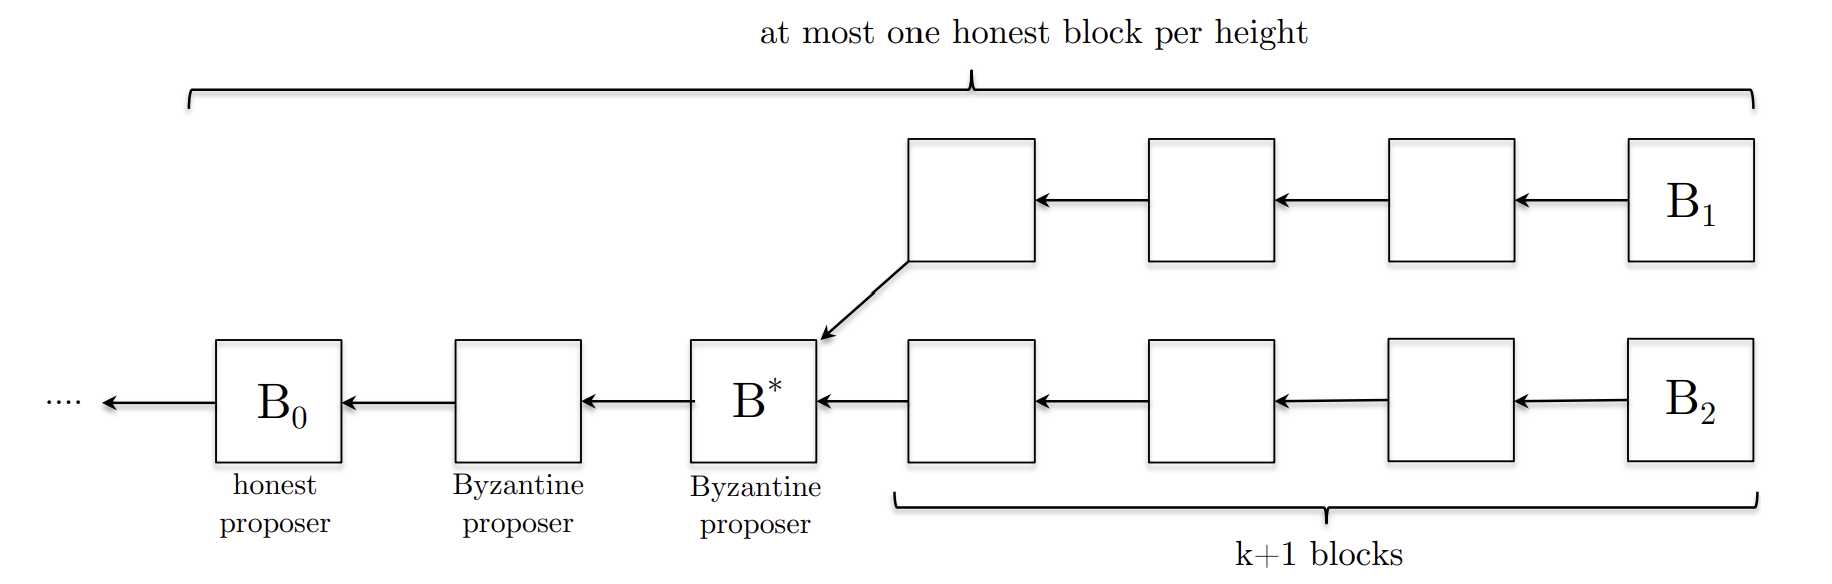
\includegraphics[scale = 0.5]{figures/f29.png}
    \caption{Proof of Theorem 8.7.1: if there are two longest chains that disagree in more than
their last $k$ blocks, the window of $ \geq 2k + 2$ leaders following the production of $B_0$ must have
been at least half Byzantine.
}
    \label{fig:mesh1}
\end{figure}\\

Let’s pause for a quick proposition. Recall that the height of a block is the number of
hops required to get back to the genesis block (equivalently, the length of the chain from the
genesis block to that block).
\mprop{Honest Blocks Having Increasing Heights}{Under assumption (A5),
the heights of honestly produced blocks are strictly increasing over time.
\begin{myproof}
Suppose that the blocks $B_i$ and $B_j$ are produced by honest leaders $i$ and $j$. There’s
only one leader per round, so one of $i$ or $j$ is chosen as a leader first—let’s say $i$, with its
block $B_i$ at height $h$. Because $i$ is honest, it announces its block $B_i$
immediately, and by
assumption (A5), node $j$ finds out about it immediately. At the subsequent round in which $j$
creates $B_j$
, because $j$ is honest, $B_j$ extends one of the longest chains that j is aware of at
that time. Because $j$ is aware of a block at height $h$ (namely, $B_i$) at that time, its block $B_j$
will have a height of at least $h + 1$.
\end{myproof}}

In particular, there cannot be two honestly produced blocks at the same height:
\cor{At Most One Honest Block Per Height}{ If assumption (A5) holds and
blocks $\hat{B}$ and $\tilde{B}$ were both produced by honest leaders, then $\hat{B}$ and $\tilde{B}$ have different heights.}

Returning to the scenario depicted in Figure 8.8, let $r_0$ denote the round (with an honest
leader) in which the block $B_0$ was created (and announced), and consider the sequence of
leaders selected in rounds after $r_0$. The plan is to prove an upper bound on the number
of honest leaders and an equal lower bound on the number of Byzantine leaders following
round $r_0$, which together show that there is a long window comprising at least 50\% Byzantine
leaders (a contradiction). So, let $h_0$, $h^*$, and $h$ denote the heights of $B_0$, $B^*$, and the ends of the longest chains ($B_1$ and $B_2$), respectively. We can finish the proof of Theorem 8.7.1 by showing that: (i) there have been at least $2k + 2$ leaders selected after round $r_0$; (ii) at most
h-$h_0$ leaders selected after round $r_0$ could have been honest; and (iii) at least $h - h_0$ leaders selected after round $r_0$ must have been Byzantine. All three of these facts follow from some
short observations:
\begin{enumerate}
    \item Because $B_0$ was only created in round $r_0$, every block with $B_0$ as an ancestor was
    created in a round subsequent to $r_0$.
    \item Because there are at least $2k + 2$ blocks with $B_0$ as an ancestor (at least $k + 1$ blocks
    each on the chains ending at $B_1$ and $B_2$), and because (by assumption (A4’)) each
    of these blocks was produced by a distinct leader, the window of leaders following
    round $r_0$ has length at least $2k + 2$.
    \item By Proposition 8.7.1 and Corollary 8.7.1, every honest leader of a round subsequent to $r_0$
    created (and announced) a block at a height greater than $h_0$, with at most one honestly
    produced block per height.
    \item Because there have been no honestly produced blocks at heights higher than $h$, the
    total number of honest leaders subsequent to round $r_0$ thus far is at most $h - h_0$.
    \item  By the definition of $B_0$, the $h^* - h_0$ blocks between $B_0$ and $B^*$
    (excluding $B_0$ but including $B^*$) were all produced by Byzantine leaders.
    \item At each height $h^* + 1, h^* + 2, \cdots , h$, at least two blocks have been produced (one on
    the chain from $B^*$
    to $B_1$, a second one on the chain from $B^*$
    to $B_2$).
    \item Because there is at most one honestly produced block per height, at each height $h^* +1, h^* + 2, \cdots , h$, there is at least one block produced by a Byzantine leader. Thus, the total number of blocks produced by Byzantine leaders after round $r_0$ is at least $(h^* - h_0) + (h - h^*) = h - h_0$.
    \item By assumption (A4’), at least $h - h_0$ distinct Byzantine leaders (after round $r_0$) were
    required to produce these blocks.
    \item Because there are at most $h - h_0$ honest leaders and at least $h - h_0$ Byzantine leaders
    after round $r_0$, the window of leaders from round $r_0$ + 1 to the current round is at least
    half Byzantine.
    \item Thus, the leader sequence is not ($2k + 2$)-balanced.
This completes the proof of Theorem 8.7.1.
\end{enumerate}

\section{Finality of Longest-Chain Consensus}
We introduced finality back in Section 8.3.4, as the consistency of an honest node with its
future self. (As opposed to consistency between different honest nodes at a given moment in
time, which is currently trivialized by our assumption (A5) but is also the easier consistency
property to establish for longest-chain consensus.) In our discussion of BFT-type consensus
protocols (chapters 2–7), the finality property was implicit in our description of the SMR
problem, in particular the “append-only” requirement for honest nodes’ local histories. As
we've seen, in longest-chain consensus, there is a very real risk of blocks getting kicked off
of the longest chain and it is not at all obvious whether finality should hold with any value
of the parameter $k$.\\
Happily, the proof of the common prefix property (Theorem 8.7.1) has already done all the
heavy lifting required to establish the finality of the longest-chain consensus. In fact, finality
reduces to the common prefix property—if the latter holds (for whatever reason), the former
automatically does as well.\\

\thm{Finality of Longest-Chain Consensus}{Let $G_1 \subseteq G_2 \subseteq \cdots\subseteq G_T$ denote a sequence of in-trees, with each in-tree $G_i$ having one more block than the previous one $G_{i-1}$. If the common prefix property (with a given value of $k$) holds in each
of $G_1, G_2, \cdots, G_T$ , then:
$$B_k(G_1) \subseteq B_k(G_2) \subseteq \cdots\subseteq B_k(G_T). \quad(5)$$
}


You should think of the sequence $G_1 \subseteq G_2 \subseteq \cdots\subseteq G_n$as the in-tree of blocks known to
(all) honest nodes at each of the rounds $1, 2,\cdots, T$. (By assumption (A5), all honest nodes
know about exactly the same blocks. Honest nodes never forget about blocks, so each in-tree
contains the previous one. If multiple blocks are announced in the same round, imagine that
they are added to the in-tree one by one in an arbitrary order.) Then, the expression (5)
asserts finality: once a block is on the longest chain with at least $k$ blocks following it (at
hence considered confirmed), it will continue to be so forevermore. Said differently, blocks
only get added to $B_k(G)$ as the current in-tree $G$ grows, never removed.
The statement of Theorem 8.8.1 does not refer to any of our assumptions (A1)–(A5), or to
any assumptions about the leader sequence. None are necessary—the proof is a simple combinatorial argument about in-trees, and it shows that as long as the common prefix property
holds throughout the sequence (for whatever reason), and finality also holds. For example, the
conclusion of Theorem 8.8.1 will hold under the same assumptions that are stated in Theorem 8.7.1.\\
\begin{figure}[h]
    \centering
    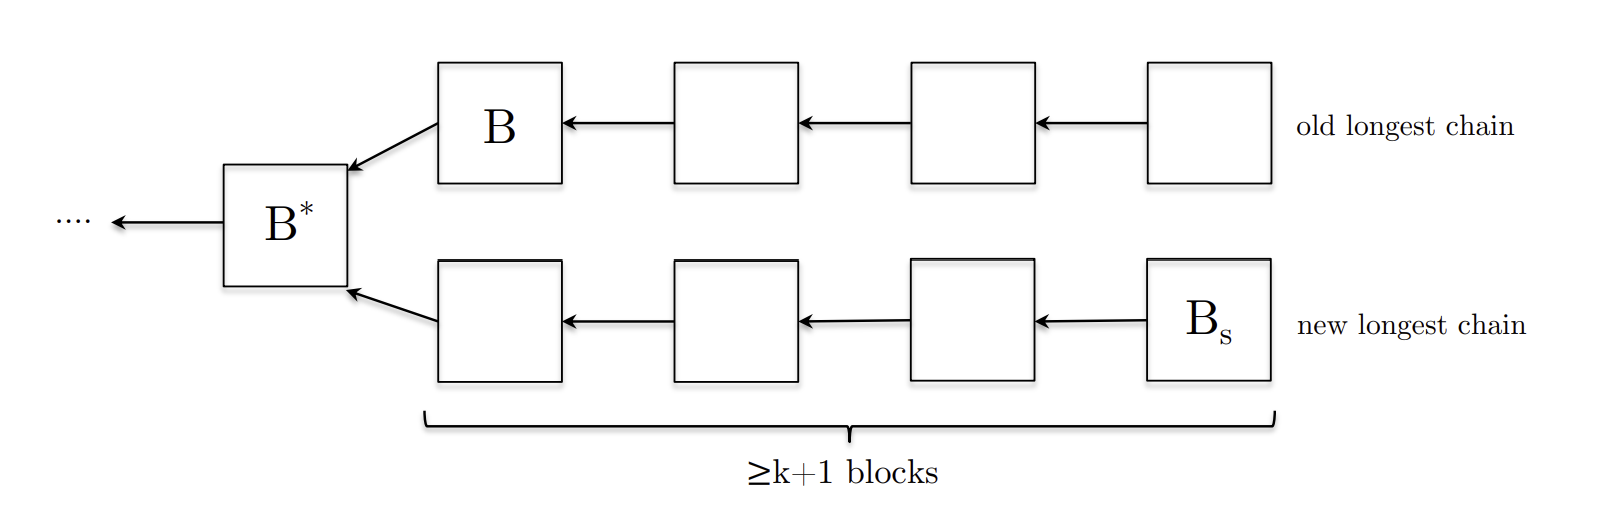
\includegraphics[scale = 0.5]{figures/f30.png}
    \caption{Proof of Theorem 8.8.1: the only way that a block that is at least $k$ blocks deep on
the longest chain can ever get rolled back is through a failure of the common prefix property.
}
    \label{fig:mesh1}
\end{figure}\\

\textit{Proof of Theorem 8.8.1:} We proceed by contradiction. Suppose that the common prefix
property (with parameter $k$) holds in each of $G_1, G_2, \cdots, G_T$ (and hence $B_k(G_i)$ is well
defined for all $i$), but that finality (5) fails. This means that there’s a block $B$ that is
confirmed at some step $i$ (i.e., $B \in B_k(G_i)$) but gets rolled back at some later step $j > i$
(i.e., $B \notin B_k(G_j)$).
Because $B \in B_k(G_i)$, the block $B$ belongs to (the common prefix of) every longest chain
of the in-tree $G_i$. Because $B \in B_k(G_j)$, there is at least one longest chain that excludes 
block B. Let $s \in \{i+1, i+2, \cdots , j\}$ denote the smallest index such that $B$ is excluded from
at least one longest chain of $G_s$. The new block $B_s$ added to $G_{s-1}$ to form $G_s$ cannot have
extended an existing longest chain (because that chain would then, like its prefix, include $B$),
so it must have created a new longest chain, tied in length with the longest chains of $G_{s-1}$
but also excluding the block $B$ (see Figure 8.9, which may look hauntingly familiar).
Pick an arbitrary longest chain $C_1$ of $G_{s-1}$ and let $C_2$ denote the chain in $G_s$ that ends
with the new block $B_s$. Both $C_1$ and $C_2$ are the longest chains of $G_s$. Because $B$ is more than $k$
blocks deep on the incumbent longest chain $C_1$ and missing from the new longest chain $C_2$,
the least common ancestor B∗ of $C_1$ and $C_2$ predates $B$ and hence is more than $k + 1$ blocks
deep on $C_1$ and $C_2$. This means that $C_1$ and $C_2$ differ in at least their last $k + 1$ blocks.
Because $C_1$ and $C_2$ are both the longest chains of $G_s$, $G_s$ must then fail to satisfy the common
prefix property, contradicting our initial assumption. This contradiction completes the proof
that the common prefix property implies finality.\\

We noticed already in Section 8.4.2 that embracing forks and resolving them in-protocol
would seem to threaten finality. So it’s pretty cool and somewhat surprising that finality
holds for longest-chain consensus under reasonably palatable assumptions (and an appropriately large value of $k$)!


\section{Liveness of Longest-Chain Consensus}

No analysis of a consensus protocol is complete without also addressing liveness, and proving
that (under our standing assumptions) progress is guaranteed. We’ll be using the same
definition of liveness that we used in the last chapter to analyze Tendermint.
\nt{\begin{center}
    \textbf{Liveness (Weak Version)}
\end{center}If a transaction is known to all honest nodes, that transaction is eventually
added to every honest node’s local history.}

We’ll establish liveness under the same balancedness condition used in our proof of the
common prefix property (Theorem 8.7.1). For the liveness analysis, we won’t need to worry
about the distinction between assumption (A4) and its stronger version (A4’)—the argument
will work assuming only (A4) and that the common prefix property holds (for whatever
reason).\\
\thm{Liveness of Longest-Chain Consensus}{If assumptions (A4) and (A5)
hold and the leader sequence $l_1, l_2, l_3,\cdots$ is sufficiently long and ($2k + 2$)-balanced, and if
the common prefix property holds in the corresponding sequence of in-trees, every transaction
that is at some point known to all honest nodes will eventually be included in $B_k(G)$, where $G$ denotes the in-tree of blocks known to (all) honest nodes.}

Because the common prefix property implies finality (see Theorem 8.8.1), the transaction in
question will belong to the set $B_k(G)$ of finalized blocks forevermore.\\

\noindent
\textit{Proof of Theorem 8.9.1:} The plan is to prove that honestly produced blocks get finalized (i.e.,
added to $B_k(G)$) infinitely often. This implies that, if a transaction $tx$ is known to all honest
nodes at some round r, there will be a future moment in time at which a block created by
an honest leader in a round after $r$ gets added to $B_k(G)$. Because an honest leader includes
all the outstanding transactions that it knows about in its block, this block will contain $tx$
(unless $tx$ already belongs to an earlier block of $B_k(G)$).\\
Next, let’s invoke the balancedness assumption on the leader sequence. Split the sequence
into groups of $2k + 2$ consecutive leaders each, and call each group an epoch. Because the
leader sequence is ($2k+2$)-balanced, every epoch contains more honest leaders than Byzantine
leaders—at worst, $k + 2$ honest leaders and $k$ Byzantine leaders.\\
Recall that the height of a block is the length of the chain from genesis to that block. The
length of the longest chain in an in-tree is therefore the same as the maximum block height.
Because we’re assuming that (A5) holds, we can invoke Proposition 8.7.2 to conclude that, in every epoch, the length of the longest chain grows by at least $k + 2$ (i.e., by at least one for
each honest node in the epoch).\\
Fast forward to the end of the $T$th epoch (for a parameter $T$), and consider a longest
chain at that time, which must contain at least $(k + 2)T$ blocks. By assumption (A4), each
Byzantine leader from the first $T$ epochs contributes at most one block to this chain. Because
at most $kT$ leaders from the first $T$ epochs were Byzantine, this longest chain contains at
least $(k + 2)T - kT = 2T$ blocks produced by honest leaders. Because the common prefix
property holds (by assumption) for the current in-tree GT of blocks known to all honest nodes,
$B_k(G_T)$ is well defined and contains at least $2T - k$ of this $ 2T$ honestly produced blocks.
Thus, as the parameter $T$ increases (and remembering that $k$ is a fixed constant like 100,
independent of $T$), honestly produced blocks must be added to $B_k(G)$ infinitely often. This
fulfills our proof plan and completes the liveness analysis of longest-chain consensus.

\section{Chain Quality of Longest-Chain Consensus}
\subsection{Stronger Liveness Guarantees}
Theorem 8.9.1 establishes the basic liveness guarantee of longest-chain consensus—under
our standing assumptions, transactions known to all honest nodes will eventually be finalized.
What else could we want? There are a few different ways we could try to strengthen this
liveness guarantee.\\
\begin{enumerate}
    \item Replace the assumption that all honest nodes know about a transaction with the
    weaker assumption from Chapter 2 that at least one honest node knows about it. As
    noted in the previous section, this stronger liveness guarantee generally doesn't hold
    for longest-chain consensus under our standing assumptions (exercise).
    \item Strengthen the “will eventually be finalized” guarantee to a quantitative guarantee
    that gives concrete bounds on latency (i.e., on time-to-finalization) as a function of the
    relevant parameters (e.g., how far the fraction $\alpha$ of Byzantine nodes/hashrate/stake is
    below 50\%). This is a quite an interesting topic, but exploring it would take us too far
    afield; see e.g. for entry points to the academic literature on such latency guarantees.
    \item Strengthen the “honest blocks get added to $B_k(G)$ infinitely often” guarantee to a
    concrete lower bound on the fraction of blocks of $B_k(G)$ that was produced by honest
    nodes (again, as a function of the relevant parameters). This fraction is known as the
    chain quality, and it is the strengthening that we will discuss here.
\end{enumerate}

If the fraction of honest nodes/hashrate/stake is barely above 50\%, the chain quality of
longest-chain consensus isn’t really any better than what Theorem 8.9.1 suggests (namely,
that the chain quality is more than 0\%). But does it help if, say, 60\% of the nodes are
honest?
\subsection{Generalizing the Proportional Representation Argument}
Let’s return to the case of randomly chosen leaders, as in Section 8.6. Recall the first two
parts of the intuition for the analysis of random leaders in Section 8.6.2 (and the corresponding
proofs in Section 8.6.3):
\begin{enumerate}
    \item 
\end{enumerate}
1. A consequence of the law of large numbers is the hopefully intuitive fact that if you
repeat an experiment with success probability $p$ a large number of times, the long-run
fraction of successes you’ll see is almost always going to be roughly $p$.
2. Identifying a successful experiment with the selection of an honest leader, means
that after enough repeated trials the long-run fraction of honest leaders is almost
always going to be roughly $1 - \alpha$, where $\alpha = \frac{f}{n}$ denotes the fraction of nodes that
are Byzantine.
In our basic analysis in Section 8.6, we then used the fact that $\alpha < \frac{1}{2}$ (and hence $\alpha < 1 - \alpha$)
to conclude that honest leaders should outnumber the Byzantine leaders in every sufficiently
large window. More generally, the exact same argument shows that the fraction of honest
leaders should be very close to $1-\alpha$ in every sufficiently large window. To make this precise:
\dfn{$(w, \rho)$-Balanced Leader Sequence}{A sequence $l_1, l_2, l_3, \cdots \in \{H, A\}$
is $(w, ρ)$-balanced if, in every window $l_i
, l_{i+1},\cdots, l_{j-1}, l_j$ of length at least $w$, the number of A’s is less than $\rho . (j - i + 1)$.}
The basic $w$-balanced condition (Definition 8.5.1) is the special case of the $(w, \rho)$-balanced
condition with $\rho = \frac{1}{2}$.\\
The hope is that if, for example, only 40\% of the nodes are Byzantine, then in every
sufficiently long window less than 41\% of the chosen leaders are Byzantine (with high probability). And indeed, the “proportional representation” analysis from Section 8.6.3, repeated
verbatim, culminates in the following analog of (4):
$$\textbf{Pr}[\text{a sequence of $T$ randomly selected leaders is $(w, \alpha + \varepsilon)$-balanced}] \geq 1 - T^2 . e^{-cw}\quad (6)$$
(The “$e^{-cw}$” failure probability term comes from the law of large numbers argument summarized in (2) and applied to a single length-$\geq w$ window, and the “$T^2$” term comes from a
Union Bound over all possible length-$\geq w$ windows.)\\

\noindent
\textbf{Glossary of notation.} In (6), $w$ is the minimum window length we’re interested in (perhaps 50 or 100), $T$ is the length of the entire leader sequence that we’re looking at (e.g.,
the leaders chosen over the course of a day or a week), $\alpha$ is the fraction of nodes that are
Byzantine (e.g., 40\%), $\varepsilon$ is a parameter of our choosing that is close to 0 (e.g., 0.1 or 0.01),
and $c$ is a constant independent of $T$, $w$, and $\alpha$ (like .1). The constant $c$ does depend on our choice of $\varepsilon$, with smaller values of $\varepsilon$ (i.e., more stringent proportional representation
demands) leading to smaller values of $c$ (i.e., a less rapid decay in the failure probability
as a function of the minimum window length w). You can think of the basic analysis from
Section 8.6.3 as the special case in which $\varepsilon = \frac{1}{2} - \alpha$.
As in Section 8.6.3, we then have:
\nt{
a sequence of T random leaders is $(w, \alpha+\varepsilon)$-balanced with probability at least
$1 - δ$, provided 
$$w \geq c_2(\ln T + \ln \frac{1}{\delta})$$}
Again, the constant $c_2$ depends on $\varepsilon$ (with $c_2$ increasing as $\varepsilon$ gets closer to 0) but is independent of all other parameters. As expected, larger minimum window lengths are required
to achieve smaller failure probabilities ($\delta$) and smaller tolerances around deviations from
proportional representation ($\varepsilon$).

\subsection{From Liveness to Chain Quality}
Now that we have our generalized balancedness condition (Definition 8.10.1), we can simply
repeat our liveness analysis (Theorem 8.9.1) to obtain a stronger chain quality guarantee.
\thm{Chain Quality of Longest-Chain Consensus}{If assumptions (A4) and
(A5) hold and the leader sequence $l_1, l_2, l_3, \cdots$ is sufficiently long and $(2k+2, \alpha+\varepsilon)$-balanced,
then the fraction of blocks on a longest chain that was produced by honest leaders is always
as least
$$\frac{1 - 2\alpha - 2\varepsilon}{1 - \alpha - \varepsilon} \quad(7)$$}
You can think of Theorem 8.9.1 as the special case of Theorem 8.10.1 in which $\alpha < \frac{1}{2}$ and $\varepsilon$ is
chosen infinitesimally smaller than $\frac{1}{2} - \varepsilon$ (so that $\alpha + \varepsilon < \frac{1}{2}$ and the fraction in (7) is just
barely positive).
For example, if 60\% of the nodes are honest (and $\varepsilon$ is small), Theorem 8.10.1 asserts that at
least roughly one-third of the blocks in $B_k(G)$ were produced by honest leaders. If two-thirds
of the nodes are honest, the chain quality improves to roughly 50\%.\\

\noindent
\textit{Proof of Theorem 8.10.1:} As in the proof of Theorem 8.9.1, break the leader sequence into
epochs that each consist of $2k + 2$ consecutive leaders. By the $(2k + 2, \alpha + \varepsilon)$-balancedness
assumption and Proposition 8.2, the length of the longest chain grows by at least $(2k +
2) · (1 - \alpha - \varepsilon)$ with every epoch (i.e., by at least one for each honest leader of the epoch).
After $T$ epochs, there are at least $(1 - \alpha - \varepsilon) · (2k + 2)T$ blocks on a longest chain, and
(by assumption (A4)) at most $(\alpha + \varepsilon) · (2k + 2)T$ of these could have been contributed by
Byzantine leaders (i.e., at most one block per such leader). This means that the fraction of
blocks on this chain that were honestly produced are at least
$$\frac{(1 - \alpha - \varepsilon) · (2k + 2)T - (\alpha + \varepsilon) · (2k + 2)T}{(1 - \alpha - \varepsilon) · (2k + 2)T} = \frac{1 - 2\alpha - 2\varepsilon}{1 - \alpha - \varepsilon}$$
as promised.

\subsection{Chain Quality and Selfish Mining}
How should you feel about the chain quality guarantee in (7)? The good news is that as $\alpha$
tends to 0, the chain quality tends to 100\%. On the other hand, it’s a bit disappointing that
with 67\% honest nodes Theorem 8.10.1 promises only a chain guarantee of 50\%, rather than
67\%. Shouldn't honest nodes get their fair share of blocks on the longest chain? Maybe we
can be smarter and rework the proof of Theorem 8.10.1 so that its chain quality guarantee of
(roughly) $\frac{1 - 2\alpha}{1 - \alpha}$ improves to $1 - \alpha$?\\
Alas, with arbitrary Byzantine strategies and arbitrary tie-breaking by honest nodes, the
analysis of the chain quality of longest-chain consensus in Theorem 8.10.1 is tight—for any
$\alpha < \frac{1}{2}$, the chain quality might be as low as $\frac{1 - 2\alpha}{1 - \alpha}$. We’ll see proof of this fact
in chapter 10 in the context of “selfish mining,” which is a specific strategy by Byzantine
nodes (involving the delayed announcements of blocks) designed to kick as many honestly
produced blocks off the longest chain as possible.\\
It is possible to add a bit more complexity to longest-chain consensus so that the chain
quality is guaranteed to be roughly $1 - \alpha$ (in addition to consistency and liveness in the
synchronous model whenever $\alpha < \frac{1}{2}$).
\section{ Longest-Chain Consensus in the Partially Synchronous Model}

\subsection{Partial Synchrony}
This entire chapter we've been operating under assumption (A5), meaning that all communication between honest nodes happens instantly (equivalently, the synchronous model with
delay parameter $\Delta = 0$). In Chapter 9 we’ll see why all of Theorems 8.7.1, 8.8.1, 8.9.1, and 8.10.1
extend to the synchronous model with minimal loss, provided the maximum network delay $\Delta$
is much smaller than the typical duration of a round. That’s great, but at the same time, Tendermint (chapter 7) spoiled us by offering consistency (always) and liveness (eventually)
in the more realistic partially synchronous setting, meaning even in the presence of denial-of-service attacks and network partitions. What guarantees are offered by longest-chain
consensus here?
More formally, recall (from Chapter 6) that the partially synchronous model assumes a
global shared clock and involves two parameters, an unknown global stabilization time (GST)
and a known bound $\Delta$ on the maximum message delay after GST has passed. (Intuitively,
the network begins under attack, the attack eventually ends, and after that, the network
resumes normal operation.) Before GST has passed—and nobody knows whether it has
passed or not, only that it will happen eventually—messages can be delayed arbitrarily.\\

\begin{figure}[h]
    \centering
    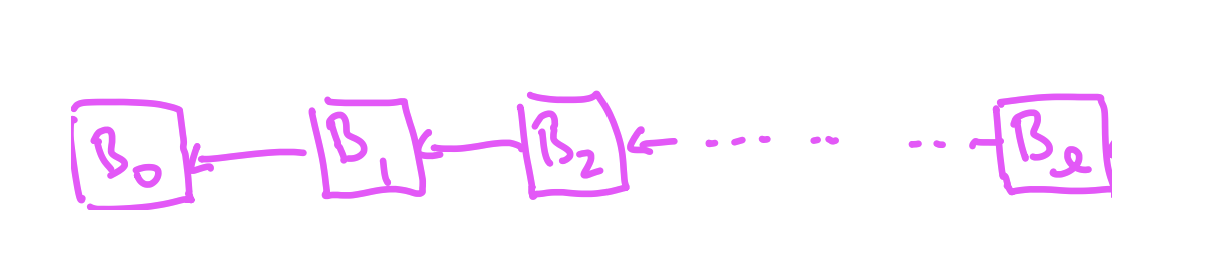
\includegraphics[scale = 0.5]{figures/f31.png}
    \caption{When there are no message delays or Byzantine nodes, there are no forks.}
    \label{fig:mesh1}
\end{figure}\\

\subsection{A Counterexample to Finality}
Longest-chain consensus breaks down badly in the partially synchronous model, unfortunately, even when there are no Byzantine nodes at all. Take finality (Theorem 9.1), for
instance, and set the security parameter $k$ as big as you like. Finality asserts that once a
block is at least $k$ blocks deep on a longest chain, it will always be at least $k$ blocks deep on
a longest chain.\\
Now imagine that longest-chain consensus (in the permissioned and PKI setting, with
no Byzantine nodes) is happily chugging along, with no forks whatsoever, producing a chain
of length $l$ (Figure 8.10) that is known to all the (honest) nodes. Suppose that we’re still
pre-GST, though, and immediately after the creation of the last block $B_l$ there is a network
partition. In a network partition (Figure 8.11)—which you might remember from our discussion of the CAP Principle in Chapter 6—the nodes are split into two groups (A and B),
with all intragroup messages delivered immediately and messages between groups delayed
indefinitely (until after GST).\\
Intuitively, in longest-chain consensus, the two sides of the network partition are going
to continue operating independently, alone in their own universes. For example, suppose
the next round is $r$, and the leader for round $r$ is a node $i$ in group A. In the permissioned
version of longest-chain consensus with the PKI assumption, everyone (both in group A and
in group B) knows that $i$ is the round-$r$ leader. Node $i$ is honest, so it dutifully produces a
block $B_{l+1}$ that extends the longest chain that it knows about and immediately announces
that block to all the other nodes. Nodes in A hear the announcement and from their
perspective, the protocol has continued to hum along normally. Nodes in B hear nothing.
From their perspective, something has gone wrong, but it’s not clear what—for example, for
all they know, node $i$ is Byzantine and never sent any block announcements to any nodes
of B.

\begin{figure}[h]
    \centering
    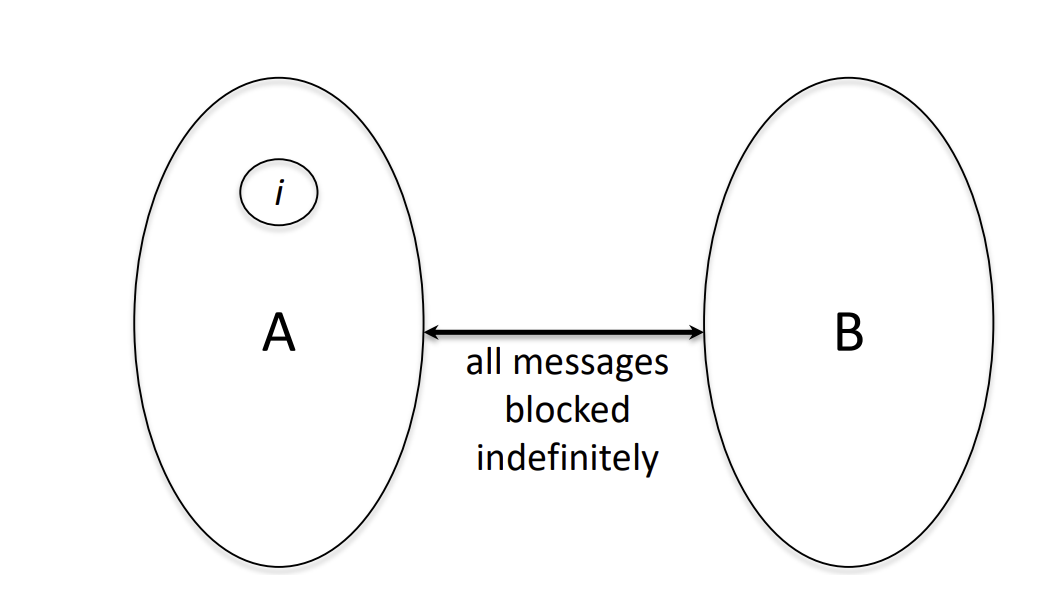
\includegraphics[scale = 0.5]{figures/f32.png}
    \caption{During a network partition (e.g., due to a denial-of-service (DoS) attack), two
disjoint sets of nodes (A and B) are unable to communicate with each other.}
    \label{fig:mesh1}
\end{figure}\\
\begin{figure}[h]
    \centering
    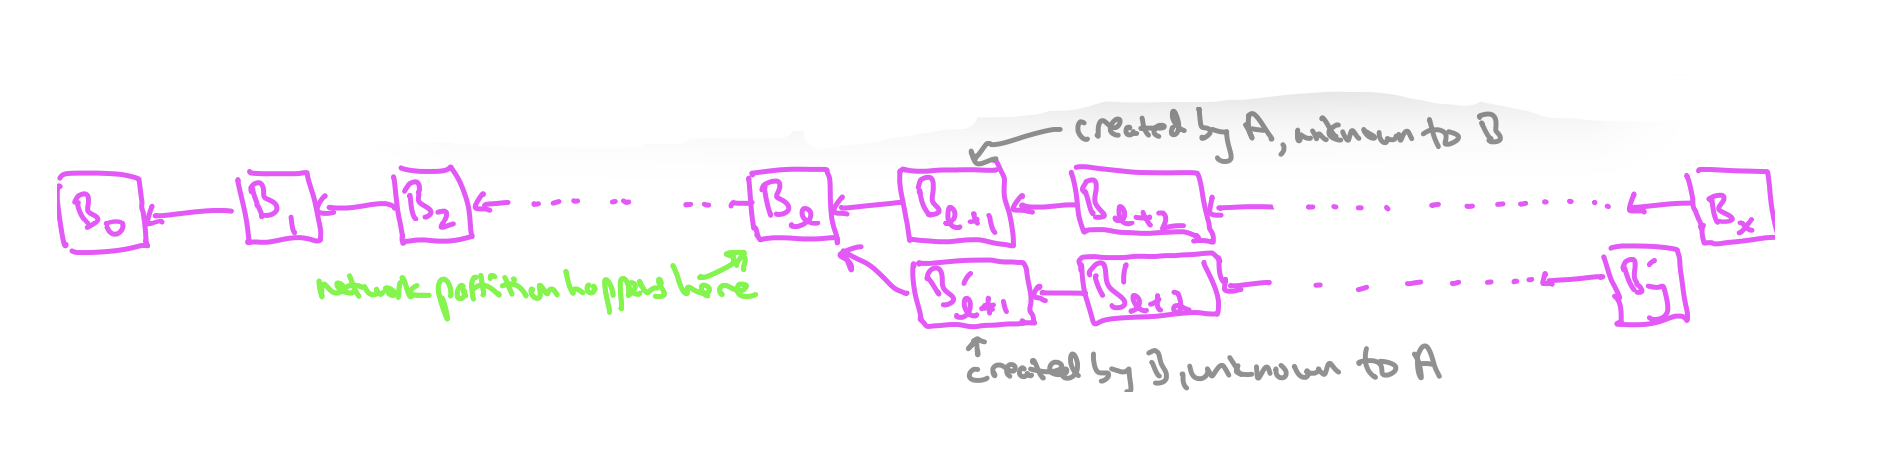
\includegraphics[scale = 0.5]{figures/f33.png}
    \caption{ With a network partition, the two sides of the partition independently create two
competing chains.}
    \label{fig:mesh1}
\end{figure}\\

At this point, nodes in group A view block $B_{l+1}$ as the end of the longest chain, while
nodes in group B don’t know about $B_{l+1}$ and think that $B_l$
is still the end of the longest
chain. Now suppose that the leader of round $r + 1$ is a node from group B. That (honest)
node will dutifully extend the longest chain that it knows about, which means that it will
produce a second block $B'_{l+1}$ that extends $B_l$. Now, even though there are no Byzantine
nodes, the blockchain has suffered a fork. The leader of round $r + 1$ will broadcast its
block $B'_{l+1}$ to everybody, but only the nodes in group B will hear about it. As long as the
network partition persists, the pattern recurs. In every round with a leader from group A, a
new block is added to the end of the top branch (the only branch that group-A nodes know
about), and similarly for leaders from group B and the bottom branch.
When the network partition eventually ends and all of the stale intergroup block announcements are delivered, all nodes will realize what the full blockchain looks like (as in
Figure 8.12). (Up to this point, every node thought that the blockchain consisted of only a
single chain.) The nodes will realize that they've been doing redundant uncoordinated work
and, worse, that the shorter of the two branches will have to be discarded.
For example, imagine that the security parameter $k$ is 50 and that the network partition
goes on so long that the nodes of groups A and B add 125 and 119 blocks to their respective
branches. (Remember GST is unknown and arbitrarily large. Thus no matter how big $k$ is chosen, a network partition can go on long enough for the creation of two competing branches
that are both longer than $k$.) The nodes in group A will breathe a sigh of relief, discard the
(shorter) competing branch, and continue with the same view of the longest chain as they
had before. The nodes in B, however, previously regarded the last $119 - k = 69$ blocks of
their branch as finalized (i.e., belonging to what they thought $B_k(G)$ was), but now all of
those blocks have to be rolled back. This is a violation of finality.

\subsection{Discussion}
The fact that longest-chain consensus fails to guarantee consistency in the partially synchronous model (in contrast to BFT-type protocols like Tendermint) is arguably its most
serious flaw. Longest-chain consensus is still useful, of course—it powers many of the
world’s biggest blockchains—but it’s important that everyone understands its weaknesses.
The breakdown of consistency in longest-chain consensus in the partially synchronous
model ties back to our discussion of fundamental consistency-liveness tradeoffs (see the FLP
impossibility result in chapters 4 & 5) and the different failure modes of different types
of blockchain consensus protocols. We know (from FLP) that we can’t guarantee both
consistency and liveness during an attack. The best we can hope for is to maintain one of
them while under attack and to recover the other quickly after the attack ends (i.e., post GST). BFT-type protocols like Tendermint guarantee consistency while under attack, so it’s
no surprise that they temporarily give up on liveness (and, for this reason, generally fail in
practice by stalling for an extended period of time).\\
Meanwhile, longest-chain consensus still has a form of liveness during a network attack.34
In our example above, 75 new blocks are finalized (and not later rolled back) during the
network partition! A BFT-type protocol, meanwhile, would finalize zero new blocks during
this time. The resiliency of liveness in longest-chain consensus during a network attack
would then suggest that consistency must be given up instead, as we verified with the
concrete counterexample above. For this reason, longest-chain blockchain protocols tend to
fail not by stalling but through large-scale chain reorganizations and the consequent reversal
of once-thought-confirmed transactions.\\
Longest-chain consensus makes very different trade-offs than BFT-type protocols and, as
such, is an innovation even from the perspective of traditional (permissioned + PKI) consensus protocols. The traditional 20th-century literature on consensus protocols focused almost
entirely on protocols that favored safety over liveness (like BFT-type protocols). It’s easy to
see why—consistency, as a safety property (i.e., bad things never happen), was historically
viewed as mission-critical and non-negotiable. Because liveness guarantees are inherently
about good things happening eventually, it was natural to allow for the “eventually” to
encompass “post-GST/attack.”\\
Longest-chain consensus shows that the classical literature was missing some interesting
and non-trivial points in the consensus protocol design space, and that favoring safety over
liveness is not the only option. If the application demands it, you can use a consensus
protocol (like longest-chain consensus) that continues to make progress when under attack,
with the understanding that some honest nodes may have to roll back some of the progress
that they thought they had made.

\section{Toward Permissionless Consensus}
\noindent
\textbf{Permissionless longest-chain consensus.} This chapter has focused on longest-chain consensus in the safe confines of the permissioned setting with the PKI assumption, for the
following reasons: (i) continuity with chapters 2–7; (ii) to focus on the basic consistency
and liveness guarantees of longest-chain consensus without worrying about the additional
challenges that arise in the permissionless setting (primarily “sybils”); (iii) to appreciate
that longest-chain consensus is an interesting part of the design space even in the classical
permissioned + PKI setting.\\

All that said, the real claim to fame for longest-chain consensus is its extensions to the
permissionless setting, in which the protocol has no idea which nodes might be running
it. This is obviously a much different scenario than traditional applications like database
replication, in which all the nodes would typically be servers bought in advance and operated
by a single entity. To viscerally appreciate the difference, I encourage you to spin up a full
node for a blockchain protocol like Bitcoin or Ethereum—no one can stop you, you can
literally just download the appropriate software and do it, right now.\\

Bitcoin’s fundamental breakthrough was a solution to permissionless consensus. This
involved both the invention of a new approach to consensus (longest-chain consensus) and
a novel method for “sybil-resistance” (called “proof-of-work”) that extends the guarantees
of longest-chain consensus from the permissioned to the permissionless setting.35 We now
understand that there are also other viable approaches to permissionless consensus, including
ones that use BFT-type consensus protocols and alternative approaches to sybil-resistance
(like “proof-of-stake”). We’ll get into much more detail on all of this in chapters 9 (for
proof-of-work) and 12 (for proof-of-stake).\\

\noindent
\textbf{The essence of the analysis.} So what prevents the description and analysis of longestchain consensus in this chapter from applying immediately to the permissionless setting?
Where in this chapter did we lean on the permissioned assumption?

The answer lies in the leader selection step of longest-chain consensus (step (2a) in the description in Section 8.2.2). The abstract description is silent on how this mapping (from rounds
to leaders) is made, in effect assuming that it’s carried out by some black box (Figure 8.13).
What properties of this black box were necessary for the proof of the basic consistency and
liveness properties in Sections 8.7–8.10? Three things:
\nt{\begin{center}
    \textbf{Required Properties of the Leader Selection Box}
\end{center}
\begin{enumerate}
    \item (Same as assumption (A2)) It is easy for all nodes to verify whether a
given node is the leader of a given round.
    \item (Same as assumption (A3)) No node can influence the probability with
which is selected as the leader of a round.
    \item (Required hypothesis for Theorems 8.7.1, 8.9.1, and 8.10.1) The sequence of
leaders are sufficiently balanced.
\end{enumerate}}\\
\begin{figure}[h]
    \centering
    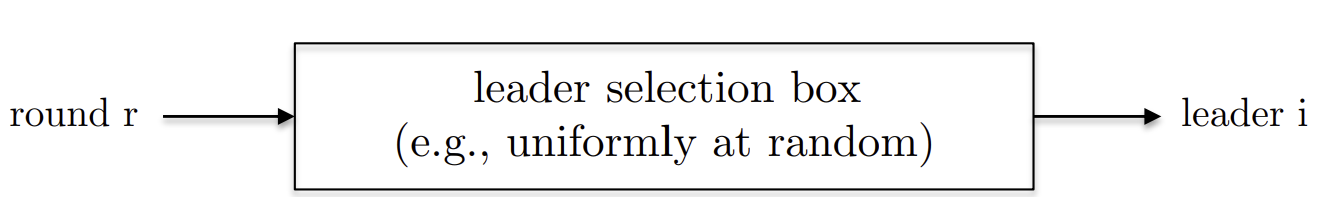
\includegraphics[scale = 0.5]{figures/f34.png}
    \caption{ Step (2a) of longest-chain consensus is effectively a black box that maps round
numbers to leader nodes.}
    \label{fig:mesh1}
\end{figure}\\
For example, the analysis in Sections 8.7–8.10 makes no reference to the number of nodes n—all
the proofs work as long as the sequence of As and Hs generated by the leader selection box
is sufficiently balanced.\\
Depending on the context, “sufficiently balanced” could mean the w-balanced condition
in Definition 8.5.1 (for Theorems 8.7.1 and 8.9.1), the version of that definition parameterized
by $\alpha$ and $\varepsilon$ (Definition 8.10.1, in service of Theorem 8.10.1). This is a
zoo of different conditions, but there’s a common sufficient condition that implies all of them
(with high probability):
\nt{
\begin{center}
    \textbf{Key Sufficient Condition for Consistency and Liveness of
Longest-Chain Analysis}
\end{center}
Leaders in different rounds are chosen independently and, in each round, the
probability that the leader is Byzantine is at most $\alpha < \frac{1}{2}$}

In other words, if you push the button on the black box to generate a new leader, the leader
that pops out is more likely, to be honest than Byzantine (with each selection independent of previous ones). This condition is the only thing we ever used in the “proportional representation” arguments in Section 8.6.3 (as you should check), and more generally it implies
all the balancedness conditions above (with high probability, and assuming that parameters
like w are chosen appropriately).\\
All the properties of longest-chain consensus that we care about (Theorems 8.7.1, 8.8.1, 8.9.1,
and 8.10.1) thus boil down to having a sufficiently balanced leader sequence, and this, in turn,
boils down to making sure that the key sufficient condition above holds. So how do we do
that?\\

\noindent
\textbf{A permissionless leader selection box?} In the permissioned setting with $n$ nodes and
the PKI assumption, the answer is straightforward: assume that the fraction $\alpha = \frac{f}{n}$ of nodes
running the protocol that are Byzantine is less than $\frac{1}{2}$, and in each round select one node
as the leader uniformly at random (with probability $\frac{1}{n}$ for each node), independently of the
other rounds.\\
Selecting a node uniformly at random would seem to be a fundamentally permissioned
idea. In the permissionless setting, where you have no idea which nodes are running the
protocol (e.g., the protocol doesn't know $n$), it’s not clear how to select a node uniformly at
random. A permissionless version of the leader selection black box, satisfying the key sufficient condition above (and also assumptions (A2) and (A3)), is thus the missing ingredient
to a permissionless version of longest-chain consensus that satisfies all of the guarantees that
we proved in this chapter. Chapter 9 presents one such permissionless black box (under the
assumption that Byzantine nodes always contribute less than half of the overall computational power devoted to the protocol) and Chapter 12 another (under the assumption that
the blockchain has a native cryptocurrency and that Byzantine nodes always contribute less
than half of the overall amount of currency that has been staked in an appropriate smart
contract). Once these permissionless leader selection boxes are in place, the consistency and
liveness guarantees from this chapter carry over immediately.\\
Hopefully, you feel like we’re close to achieving permissionless consensus with provable
consistency and liveness. And we are! Next chapter supplies (one option for) the missing
ingredient, sybil-resistance through proof-of-work.
